% !TEX TS-program = lualatex
% !BIB TS-program = biber

% \documentclass[10pt,handout]{beamer} 
\documentclass[10pt]{beamer}   

% ==============================================================================
%   THEME
% ============================================================================== 

\usetheme[progressbar=frametitle]{metropolis}

% ==============================================================================
%	CONFIG SECTION
% ============================================================================== 


% Packages

% \usepackage{appendixnumberbeamer}
% \usepackage{caption}
\usepackage{subcaption}                       % Subfigures
\usepackage{eurosym}                          % Euro symbol
\usepackage{booktabs}                         % Booktabs
\usepackage{threeparttable}                   % Tables in parts
\usepackage{tabularx}                         % Special tables
% \usepackage[scale=2]{ccicons}
% \usepackage{verbatim}
% \usepackage{pgfplots, pgfplotstable}
% \usetikzlibrary{calc}
% \usepgfplotslibrary{dateplot}
\usepackage{xspace}
\usepackage{amsmath}
\usepackage{amsthm}
\usepackage{amsfonts}
\usepackage{amssymb}
% \usepackage{stmaryrd}
\usepackage{mathtools}
\usepackage{bbold}
% \usepackage{siunitx}
% \usepackage{bbm}
% \usepackage{booktabs}
\usepackage{xcolor}
% \usepackage{fontspec}
% \usepackage{enumitem}                       % Labels in items
% \usepackage{luatexbase}                     % Fix problems of microtype
% \usepackage{microtype}
% \usepackage{pgfpages}                       % Comments notes right hand
\usepackage{hyperref}                         % Mark pdf
% \usepackage{url}                            % To cite url \howpublished in BibTeX
% \usepackage{graphics}
\usepackage{tikz}
\usepackage{wasysym}                          % Smileys
\usepackage{smartdiagram}                     % Smart diagrams like on word
\usepackage{standalone}                       % Include standlone figures
\usepackage{media9}                           % videos
% \usepackage{img/kbordermatrix}              % Label rows/columns matrix
% \usepackage{courier}                        % Required font for listings
% \usepackage{matlab-prettifier}              % Listings for code (Matlab)
\usetikzlibrary{shapes,arrows}
\usetikzlibrary{positioning}
\usetikzlibrary{calc}

% Image path + breaks
\graphicspath{{./img/}}                     % Images Folders
% \allowdisplaybreaks                         % Breaks formulas

% Custom commands for math
\DeclarePairedDelimiter\abs{\lvert}{\rvert}
\DeclarePairedDelimiter\norm{\lVert}{\rVert}
\DeclarePairedDelimiter\floor{\lfloor}{\rfloor}

% Custom commmands for tabularx
\newcolumntype{C}{>{\centering\arraybackslash}X}
\newcolumntype{L}{>{\raggedright\arraybackslash}X}

% \theoremstyle{plain}
% \newtheorem{proposition}{Proposition}

\newcommand{\mySet}[1]{\mathcal{#1}}
\newcommand{\roads}{\mySet{R}}
\newcommand{\roadsin}{\mySet{R}^\text{in}}
\newcommand{\roadsout}{\mySet{R}^\text{out}}
\newcommand{\intersection}{\mySet{I}}
\newcommand{\neighUp}{\mathcal{N}^-}
\newcommand{\neighDown}{\mathcal{N}^+}
\newcommand{\laplacian}{\mathcal{L}}
\newcommand{\Malpha}{\overline{u}}

\newtheorem{asm}{Assumption}
\newtheorem{dfn}{Definition}
\newtheorem{prp}{Proposition}
\newcommand{\arrivallane}{\ell+}
\newcommand{\departurelane}{\ell-}
\newcommand{\lane}{\ell}
\newcommand{\scrpt}[3]{{#1}^{#2}_{#3}}    
\newcommand{\tim}[2]{t^{#1}_{#2}}        
\newcommand{\pos}[2]{x^{#1}_{#2}} 
\newcommand{\pnt}[2]{g^{#1}_{#2}}     
% \newcommand{\norm}[1]{\left\lVert#1\right\rVert}
\DeclareMathOperator*{\argmax}{arg\,max}
\DeclareMathOperator*{\argmin}{arg\,min}

% Colorsetting
\definecolor{calpolypomonagreen}{rgb}{0.12, 0.3, 0.17}

% \newcommand{\tr}[1]{\color{red}{#1}}
% \newcommand{\tg}[1]{\color{green}{#1}}
% \newcommand{\tb}[1]{\color{blue}{#1}}

% PDF marks
\hypersetup{
  pdfauthor={Andres Ladino},
  pdftitle={Control in Traffic Networks},
  pdfsubject={ITS Course},
  urlcolor=blue,
}

% Bibliography setups
% \AtBeginBibliography{\footnotesize}
% \AtBeginNote{%
%     \let\enumerate\itemize%
%     \let\endenumerate\enditemize%
% }
 

\usepackage[style=verbose,backend=biber,url=false,doi=false]{biblatex}
\addbibresource{bibliography.bib}
\addbibresource{references.bib}

% Metadata
\title[Control of Traffic Networks]{Control for transportation\\ vehicle \& urban traffic networks}
\subtitle{Course: Intelligent Transportation Systems (ITS)\\ ITS for Smart Mobility}
\date{Lyon, 4th December 2019}
\author{\texorpdfstring{Andres Ladino\newline\url{http://bit.ly/ITS2019-Control}\newline\url{andres.ladino@ifsttar.fr}}{}}
\institute{Institute Fran\c{c}ais des Sciences des Transports, de l'Am\'{e}nagement et des R\'{e}seaux (IFSTTAR)} \titlegraphic{\hfill\includegraphics[height=1.5cm]{logo.png}}


\begin{document}

\maketitle

% use <handout:1|beamer:0> to include on handout/exclude on presentation

\begin{frame}
\frametitle{Team \& Expertise}
    \begin{columns}
        \column{0.35\textwidth}
        \begin{figure}
        \centering
        \includegraphics[width=\textwidth]{fig_30_licit.png}
        \end{figure}
        \column{0.65\textwidth}
        \begin{itemize}
        \item \textbf{Modeling \& Characterization}
            \begin{itemize}
            \item Multi network traffic approach\\
                    {\scriptsize mode, physical, scale, criteria}
            \item Cooperation and autonomous vehicles 
                    {\scriptsize CAV - platooning}
            \item Realtime operations\\ 
                    {\scriptsize Short-term traffic forecast}
            \end{itemize}
        \uncover<2->{
        \item \textbf{Optimal \& decision making}
            \begin{itemize}
            \item Model optimization via\\ 
                    {\scriptsize Dynamic control, route choice}
            \item Integrated \& hierarchical control\\
                    {\scriptsize Tactical, operational}                
            \item Demand management\\
                    {\scriptsize Dynamic traffic assignment}             
            \end{itemize}
        }
        \end{itemize}
    \end{columns}
\end{frame} % Team and expertise

\begin{frame}
\frametitle{Opportunities \& Partnerships}
    \begin{columns}
        \column{0.3\textwidth}
        \begin{figure}
        \centering
        \includegraphics[width=\linewidth]{fig_28_symuvia}
        \caption{Traffic simulation in Symuvia}
        \end{figure}
        \column{0.6\textwidth}
        \begin{example}
        \begin{itemize}
            \item \textbf{SymuVia:} Inhouse simulator \(\rightarrow\)Open Source
            \item \textbf{Transpolis:} Field Operational Tests  
            \begin{itemize}
            \item Autonomous vehicles 
            \item Controlled tests 
            \item C-ITS services
            \end{itemize}
        \end{itemize}
        \end{example} 
    \end{columns}
    \begin{columns}
        \column{0.5\textwidth}
        \begin{figure}
        \centering
        \includegraphics[width=\linewidth]{fig_31_transpolice}
        \end{figure}
        \column{0.5\textwidth}
        \begin{figure}
        \centering
        \includegraphics[width=0.6\linewidth]{fig_29_transpolice}
        \end{figure}    
    \end{columns}
\end{frame} % Partners and opportunities 

\begin{frame}
\frametitle{Motivation}
\framesubtitle{Traffic research}
    Top-companies investing in R\&D on road traffic management
    \begin{figure}
      \begin{subfigure}[c]{.2\paperwidth}
      \centering
      \includegraphics[scale=0.06]{fig_34_tomtom}
      \end{subfigure}
      \begin{subfigure}[c]{.2\paperwidth}
      \centering
      \includegraphics[scale=0.125]{fig_33_here}
      \end{subfigure}
      \begin{subfigure}[c]{.2\paperwidth}
      \centering
      \includegraphics[scale=0.125]{fig_32_google_maps}
      \end{subfigure}
      \begin{subfigure}[c]{.2\paperwidth}
      \centering
      \includegraphics[scale=0.125]{fig_36_facebook}
      \end{subfigure}
    \end{figure}
    \uncover<2->{
    \begin{figure}
     \includegraphics[scale=0.3,clip,trim={2.3cm 1cm 0 1cm}]{fig_35_investments}
    \end{figure}
    }
    % \begin{center}
    % EU investments in transportation (2014)\\[1em]
    % \begin{tikzpicture}[scale=.75]
    % \node at (-0.5,.25) {All};
    % \node at (-0.5,-.75) {Sea};
    % \node at (-0.5,-1.75) {Air};
    % \node at (-0.5,-2.75) {Rail};
    % \node at (-0.5,-3.75) {Road};
    % \draw[fill=red] (0,0) rectangle (10,0.5) node [midway] {\textbf{101.7 Billion \euro}};
    % \draw[fill=blue!80!white] (0,-1) rectangle (0.54,-0.5) node [midway]{\textbf{5.4}};
    % \draw[fill=blue!80!white] (0.54,-2) rectangle (1.27,-1.5) node [midway] {\textbf{5.7}};
    % \draw[fill=blue!80!white] (1.27,-3) rectangle (4.785,-2.5) node [midway] {\textbf{37.21}};
    % \draw[fill=blue!80!white] (4.785,-4) rectangle (10,-3.5) node [midway] {\textbf{53.39}};
    % \end{tikzpicture}
    % \end{center}
\end{frame} % Motivation and traffic problem 

\begin{frame}[t]
\frametitle{Some traffic statistics \dots}
    Are we improving the conditions?
    \hspace{-0.1cm}
    \begin{center}
    \begin{columns}[t]
      \begin{column}{0.5\textwidth}
      \begin{figure}
      \includegraphics[width = 0.9\textwidth]{fig_37_grenoble-traffic}
      \end{figure}
      \metroset{block=fill}
      \uncover<2->{
      \begin{alertblock}{Now $\rightarrow$}
        \begin{itemize}
          \item[\frownie] {\small Cities tend to get more urban.}
          \item[\smiley] {\small Big sources of data.}
          \item[\smiley] {\small New measurements available for this purpose (e.g. GPS).}
        \end{itemize}
      \end{alertblock}
      }
    \end{column}
    \begin{column}{0.5\textwidth}
    \uncover<3>{
      \begin{exampleblock}{Inrix}
      Lyon: In 2014 drivers waste 36.03 (40H \~ 2013) hours per year in traffic,
      Worst Hour = Tuesday 08:00-09:00 \footnote[frame]{\href{http://inrix.com/press-releases/2661/}{INRIX Report 2014}}
      \end{exampleblock}
      \begin{alertblock}{Current condition!}
      France has moved from 4th to 7th position in the list of most congested countries in Europe with 29 lost hours in congestion during congestions in 2014 -  6th in the last report in 2016\footnote[frame]{\href{http://inrix.com/press-releases/scorecard-report-france/}{INRIX Report 2015}}.
      \end{alertblock}
    }
      \end{column}
    \end{columns}
    \end{center}
\end{frame} % Some traffic stats 

\begin{frame}[t]
\frametitle{Motivation \& Current trends\dots}
    Evolution of new technologies
    \hspace{-0.5cm}
    \begin{center}
    \begin{columns}[t]
        \begin{column}{0.5\textwidth}   
        \uncover<2->{           
            \begin{figure}
                \includegraphics[width = 0.9\textwidth]{fig_38_adas}
            \end{figure}
        }
        \uncover<3>{              
            \begin{figure}
                \includegraphics[width = 0.9\textwidth]{fig_39_radar_detection}
            \end{figure} 
        }           
        \end{column}
        \begin{column}{0.5\textwidth}   
        \vspace{-0.75cm}            
        \uncover<2->{         
        \begin{exampleblock}{Current trends}
            \begin{enumerate}
                \item Development of \emph{Small Network Sensors}
                \item From \emph{Infrastructure} towards \emph{Vehicle services}
                \item Introduction of automation 
            \end{enumerate}
        \end{exampleblock}
        }
        \uncover<3>{         
        \begin{exampleblock}{Current needs}
            \begin{enumerate}
                \item \emph{Standardization}: Technologies \& services
                \item \emph{Certification}: Testing and regulation
                \item \emph{Modality}: Efficient network exploitation
            \end{enumerate}            
        \end{exampleblock}
        }
        \end{column}
    \end{columns}
    \end{center}
\end{frame} % Current trends 

\begin{frame}
\frametitle{Big challenge\dots}
\begin{figure}
    \includegraphics[width = 0.8\textwidth]{fig_40_ghg}
    \caption{Green house emissions change due to transportation from 1990-2005}
\end{figure}
\end{frame} % Big challenge 

\begin{frame}
\frametitle{Big challenge\dots}
\begin{columns}[t]
    \begin{column}{0.5\textwidth}   
    \uncover<1->{                   
    \begin{exampleblock}{GHG Emissions up to the date}
        \begin{enumerate}
            \item From 1990-2005 the relative increase in \emph{GHG} is still important
            \item Policies have been adopted EURO1-EURO6
        \end{enumerate}
    \end{exampleblock}
    }
    \end{column}
    \begin{column}{0.5\textwidth}   
    \uncover<2->{         
        \begin{exampleblock}{On the other hand}
            \begin{enumerate}
                \item \emph{Standardization}: Technologies are reaching efficiency limtits for fosil fuel
                \item \emph{Certification}: New alternative energies on the market
                \item \emph{Modality}: We understand mobility in a different way
            \end{enumerate}            
        \end{exampleblock}
        }        
    \end{column}
\end{columns}
\metroset{block=fill}
\uncover<3->{
\begin{alertblock}{Potential on new technologies}
    \vspace{0.2cm}
    There is potential on new \emph{ITS systems} that may provide new capabilities and improve efficiency leveraged by new technologies such as \emph{data, models and automation}.  
\end{alertblock}
}
\end{frame} % Big challenge - bullets 

\begin{frame}
\frametitle{General outline}
\begin{exampleblock}{Topics for today}
    \begin{enumerate}
        \uncover<1->{
        \item Introduction to: Automation in transportation systems.  
            \begin{itemize}
                \item Models in transportation and current technologies 
            \end{itemize}
        }
        \uncover<2->{
        \item Traffic control from infrastructure point of view. 
            \begin{itemize}
                \item Control of traffic lights 
                \item Scalable control laws for traffic networks
            \end{itemize}
        }
        \uncover<3->{
        \item Vehicle control to improve traffic network performance. 
            \begin{itemize}
                \item Connected vehicles and connected infrastructures
                \item Vehicle platooning and vehicle automation. 
            \end{itemize}
        }
    \end{enumerate}
\end{exampleblock}
\end{frame} % Outline 

\begin{frame}
    \frametitle{Basic concepts of control}
    \tikzstyle{block} = [draw, fill=blue!20, rectangle, minimum height=3em, minimum width=6em]
    \tikzstyle{system} = [draw, fill=red!20, rectangle, minimum height=3em, minimum width=6em]
    \tikzstyle{interface} = [draw, fill=green!20, rectangle, minimum height=3em, minimum width=6em]
    \tikzstyle{sum} = [draw, fill=blue!20, circle, node distance=1cm]
    \tikzstyle{input} = [coordinate]
    \tikzstyle{output} = [coordinate]
    \tikzstyle{pinstyle} = [pin edge={to-,thin,black}]
    \begin{center}
    \begin{tikzpicture}[auto, node distance=2cm,>=latex']
      \uncover<3->{\node [block] (controller) {Controller};}
      \uncover<5->{\node [interface, right of=controller,node distance=3cm] (actuator) {Actuator};}
      \uncover<1->{\node [system, right of=actuator, pin={[pinstyle]above:Disturbances}, node distance=3cm] (system) {System};}
      \uncover<6->{\draw [->] (controller) -- node[name=u] {$u$} (actuator);}
      \uncover<6->{\draw [->] (actuator) -- node[name=u] {$u_a$} (system);}
      \uncover<3->{\node [output, right of=system] (output) {};}
      \uncover<2->{\node [interface, below of=u] (measurements) {Sensor};}
      \uncover<2->{\draw [->] (system) -- node [name=y] {$y$}(output);}
      \uncover<2->{\draw [->] (y) |- (measurements);}
      \uncover<4->{\draw [->] (measurements) -| node[pos=0.99] {}
    node [near end] {$y_m$} (controller);}
    \end{tikzpicture}
    \end{center}
    \begin{columns}
    \uncover<3->{\begin{column}{0.4\textwidth}
    \begin{itemize}
      %\item $r$ - Reference to be tracked
      %\item $e$ - Error
      \item $u$ - Control input
      \item $u_a$ - Actuation input
      \item $y$ - Output system
    \end{itemize}
    \end{column}
    \begin{column}{0.6\textwidth}
      \begin{exampleblock}{Objective}
      \begin{itemize}
        \item Track a particular value in the output of the system.
        \item Regularize a value in the output (Stabilize).
    \end{itemize}
      \end{exampleblock}
    \end{column}}
    \end{columns}
    \end{frame} % Basic intro control 

\begin{frame}
    \frametitle{Control approach to traffic systems \dots}
    \newcommand*\nodeonecolor{}
    \newcommand*\nodesecondcolor{}
    \only<2>{\renewcommand*\nodeonecolor{blue}}  
    \only<3>{\renewcommand*\nodesecondcolor{blue}}  
    \begin{center}
    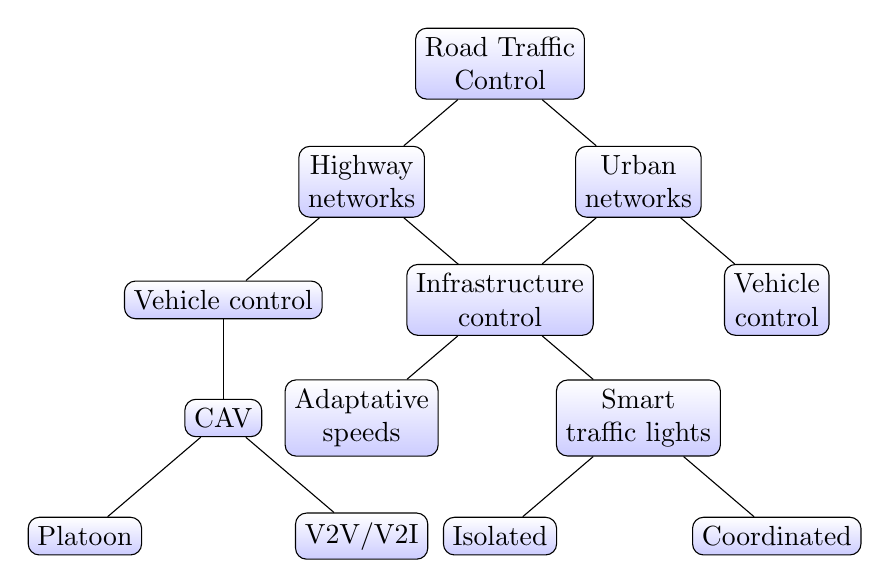
\begin{tikzpicture}[sibling distance=10em,
    every node/.style = {shape=rectangle, rounded corners,
    draw, align=center,
    top color=white, bottom color=blue!20}]]
    \node {Road Traffic\\Control}
    child { 
        node [\nodesecondcolor]{Highway\\networks}
        child{
            node [\nodesecondcolor]{Vehicle control} 
            child{
                node [\nodesecondcolor]{CAV}
                child{
                    node [\nodesecondcolor]{Platoon}
                }
                child{
                    node [\nodesecondcolor]{V2V/V2I}
                }
            }
        } 
        child{
            node {Space control}
        }
    }
    child { 
        node [\nodeonecolor]{Urban\\networks}
        child { 
            node [\nodeonecolor]{Infrastructure\\control}
            child{ 
                node {Adaptative\\speeds} 
            }
        child{ 
            node [\nodeonecolor]{Smart\\ traffic lights}
            child { 
                node {Isolated} 
            }
            child { 
                node [\nodeonecolor]{Coordinated} 
                } 
            } 
        }
        child { 
            node {Vehicle\\control}
        } 
    };
    \end{tikzpicture}
    \end{center}
\end{frame}
 % Approach to control systems 

\begin{frame}
\frametitle{Disclaimer about today's talk}
    Good solutions for mobility:
    \begin{center}
    \begin{columns}
        \begin{column}{0.3\textwidth}  
        \begin{figure}[htbp]
            \centering
            \includegraphics[width = 0.8\textwidth]{fig_41_bikesharing}
            \caption{Bikesharing}
        \end{figure}
        \end{column}
        \begin{column}{0.3\textwidth}  
        \begin{figure}[htbp]
            \centering
            \includegraphics[width = 0.8\textwidth]{fig_42_carsharing}          
            \caption{Carsharing}          
        \end{figure}
        \end{column}
        \begin{column}{0.3\textwidth}  
        \begin{figure}[htbp]
            \centering
            \includegraphics[width = 0.8\textwidth]{fig_43_ridesharing} 
            \caption{Ridesharing}                                 
        \end{figure}
        \end{column}                
    \end{columns}
    \end{center}    
    \metroset{block=fill}
    \begin{exampleblock}{Alternative Intelligent Transportation Systems}
        \begin{itemize}
            \item Leveraged by data and incentives.
            \item Complex but interesting algorithms for \emph{Dynamic traffic assignment}
            \item Sorry \frownie\ not the topic for today, but these are efficient systems from \emph{user's} point of view.
            \item Focus of today is \emph{single} mode transport optimization 
        \end{itemize}
    \end{exampleblock}


\end{frame} % Disclaimer (Shared systems)

\section{Traffic light control}

\begin{frame}
    \frametitle{Motivation}
    Scope for traffic light control:
    \begin{itemize}
      \item Focus: Urban area networks.
      \item Objective: Improve urban traffic conditions via control of traffic light (Macroscopic approach) \footcite{grandinetti2015}.
      \item How: Efficient and distributed optimization methods for the aforementioned problems \footcite{grandinetti2015a}.
    \end{itemize}
\end{frame} % Intro + references on traffic light control 

\begin{frame}
    \frametitle{Light control in traffic networks}
    \tikzstyle{block} = [draw, fill=blue!20, rectangle, minimum height=3em, minimum width=6em]
    \tikzstyle{system} = [draw, fill=red!20, rectangle, minimum height=3em, minimum width=6em]
    \tikzstyle{interface} = [draw, fill=green!20, rectangle, minimum height=3em, minimum width=6em]
    \tikzstyle{sum} = [draw, fill=blue!20, circle, node distance=1cm]
    \tikzstyle{input} = [coordinate]
    \tikzstyle{output} = [coordinate]
    \tikzstyle{pinstyle} = [pin edge={to-,thin,black}]
    \begin{center}
    \begin{tikzpicture}[auto, node distance=2cm,>=latex']
      \node [block] (controller) {Controller};
      \node [interface, right of=controller,node distance=2.5cm] (actuator) {Lights};
      \node [system, right of=actuator, pin={[pinstyle]above:Disturbances}, node distance=4cm] (system) {Traffic Network};
      \draw [->] (controller) -- node[name=u] {$u$} (actuator);
      \draw [->] (actuator) -- node[name=u] {$u_a={\color{red}0},{\color{green}1}$} (system);
      \node [output, right of=system, node distance = 2.5cm] (output) {};
      \node [interface, below of=u] (measurements) {Sensors};
      \draw [->] (system) -- node [name=y] {$y = \rho,f$}(output);
      \draw [->] (y) |- (measurements);
      \draw [->] (measurements) -| node[pos=0.99] {}
    node [near end] {$y_m$} (controller);
    \end{tikzpicture}
    \end{center}
    \begin{columns}
    \begin{column}{0.5\textwidth}
    \begin{itemize}
      \item $u$ - Green times / Red times
      \item $u_a$ - Actuation input (Green/Red)
      \item $y$ - Output system (Densities, Flows)
    \end{itemize}
    \end{column}
    \begin{column}{0.5\textwidth}
      \begin{exampleblock}{Objective}
      \begin{itemize}
        \item Alleviate congestions over the network.
        \item Adapt green times based on measurements.
    \end{itemize}
      \end{exampleblock}
    \end{column}
    \end{columns}
\end{frame} % Light control in traffic networks

\begin{frame}
    \frametitle{Urban vs Highway model}
    \begin{columns}[c]
    \column{0.4\textwidth}
    \includegraphics<1->[scale=0.25]{fig_45_high}
    \column{0.4\textwidth}
    \includegraphics<1->[scale=0.13]{fig_44_grenoble}
    \end{columns}

    \begin{block}<2->{Topology gap}
    \begin{itemize}
    \item Control strategies from \emph{highways} can be \emph{adapted} to urban cases?
    \item Is it possible to design control for the full network?
    \end{itemize}
    \end{block}
\end{frame} % Urban scenarios vs highway (complexity)

\begin{frame}[shrink=8]
    \frametitle{Traffic light modeling}
    \metroset{block=fill}
    \uncover<1->{
    \begin{block}{Two level of complexity}
    \begin{itemize}
    \item Size of the network's model
    \item Traffic light almost each intersection
    \end{itemize}
    \end{block}
    }
    \begin{columns}
    \column{0.45\textwidth}
    \uncover<2->{
    \begin{block}{Piece--wise system representation}
    \begin{center}
    \includegraphics[scale=0.55]{fig_46_intersection}
    \end{center}
    CTM still possible (each road is a cell) but the choice Free/Congested can give dimensional problem ($\sim 2^{\symbol{35}\mbox{roads}}$)
    \end{block}
    }
    \column{0.45\textwidth}
    \uncover<3->{
    \begin{block}{Discontinuities in traffic signal}
    \begin{center}
    \includegraphics[scale=0.65]{fig_47_light-plot}
    \end{center}
    A traffic light is a $T$--periodic, discontinuous signal $u(t)\in\{{\color{red}0},{\color{green}1}\}$, with duty cycle $\frac{1}{T}\int_0^T u(t) \onslide<2->{ = \frac{\overline{u}}{T}}$
    \end{block}
    }
    \end{columns}
\end{frame} % Levels of complexity 

\begin{frame}
    \frametitle{Traffic light control}
    \begin{center}
    \resizebox{!}{0.7\textwidth}{%
    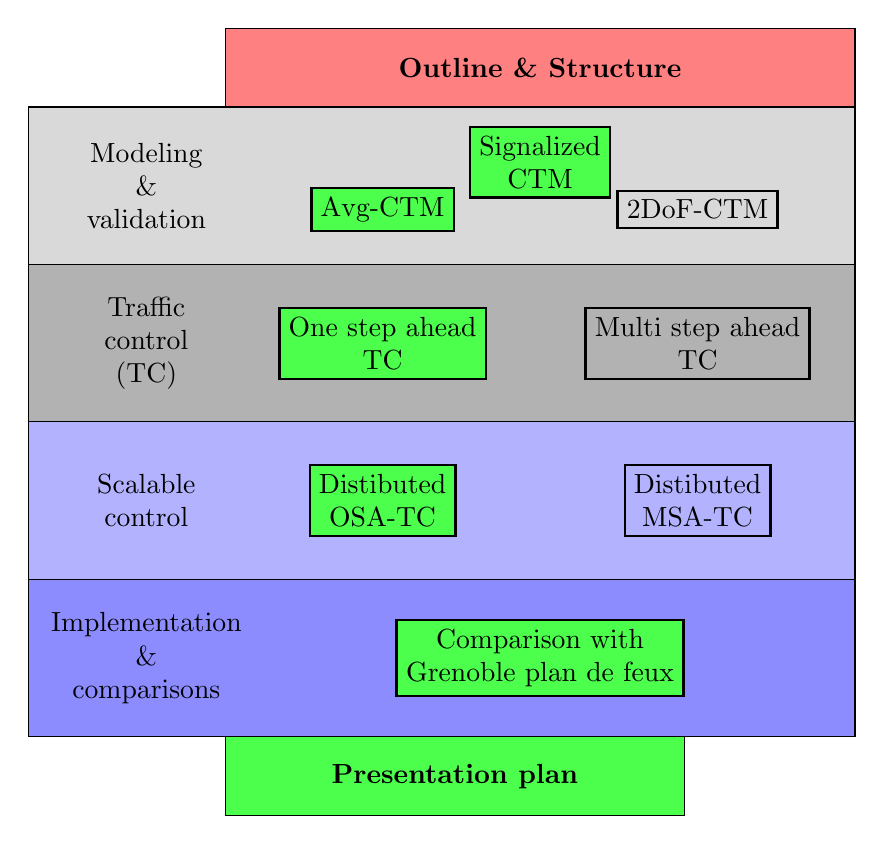
\begin{tikzpicture}
    \draw[black, fill=gray!30!white] (-0.5,0) rectangle (10,-2);
    \node[align=center] at (1,-1) {Modeling \\ \& \\ validation};
    %
    \draw[black, fill=gray!60!white] (-0.5,-2) rectangle (10,-4);
    \node[align=center] at (1,-3) {Traffic \\ estimation \\ (TE)};
    %
    \draw[black, fill=gray!60!white] (-0.5,-2) rectangle (10,-4);
    \node[align=center] at (1,-3) {Traffic \\ control \\ (TC)};
    %
    \draw[black, fill=blue!30!white] (-0.5,-4) rectangle (10,-6);
    \node[align=center] at (1,-5) {Scalable \\ control};
    %
    \draw[black, fill=blue!45!white] (-0.5,-6) rectangle (10,-8);
    \node[align=center] at (1,-7) {Implementation \\ \& \\ comparisons};
    %

    \draw[black, fill=red!50!white] (2,0) rectangle (10,1) node[midway] {\textbf{Outline \& Structure}};
    \uncover<2->{
      \node[draw,thick,align=center] at (6,-.7) {Signalized\\CTM};
      \node[draw,thick,align=center] at (4,-1.3) {Avg-CTM};
      \node[draw,thick,align=center] at (8,-1.3) {2DoF-CTM};
    }
    \uncover<3->{
      \node[draw,thick,align=center] at (4,-3) {One step ahead\\TC};
      \node[draw,thick,align=center] at (8,-3) {Multi step ahead\\TC};
    }
    \uncover<4->{
      \node[draw,thick,align=center] at (4,-5) {Distibuted\\OSA-TC};
      \node[draw,thick,align=center] at (8,-5) {Distibuted\\MSA-TC};
    }
    \uncover<5->{
      \node[draw,thick,align=center] (PdF) at (6,-7) {Comparison with\\ Grenoble \emph{plan de feux}};
    }
    \coordinate (tmp) at (PdF.east);
    \uncover<6->{
      \draw[black, fill=green!70!white] let \p1=(tmp) in (2,-8) rectangle (\x1,-9) node[midway] {\textbf{Presentation plan}};
      \node[draw,thick,align=center,fill=green!70!white] at (6,-.7) {Signalized\\CTM};
      \node[draw,thick,align=center,fill=green!70!white] at (4,-1.3) {Avg-CTM};
      \node[draw,thick,align=center,fill=green!70!white] at (4,-3) {One step ahead\\TC};
      \node[draw,thick,align=center,fill=green!70!white] at (4,-5) {Distibuted\\OSA-TC};
      \node[draw,thick,align=center, fill=green!70!white] at (6,-7) {Comparison with\\ Grenoble plan de feux};
    }
    \end{tikzpicture}
    }
    \end{center}
\end{frame}
 % Traffic light outline 

\begin{frame}
    \frametitle{The signalized cell transmission model (S-CTM)}
    \begin{minipage}[c]{0.4\textwidth}
    CTM properties:
    \begin{itemize}
    \item Macroscopic model
    \item Network partitioned into cells
    \end{itemize}
    \end{minipage}
    ~
    \begin{minipage}[c]{0.4\textwidth}
    \uncover<2->{
    \begin{tabular}{cc}
    \toprule
    Notation & Value\\
    \midrule
    $\rho_i^\text{max}$ & Cell $i$ jam density\\
    $v_i$ & Free-flow speed\\
    $w_i$ & Congestion wave speed\\
    $f_i^\text{max}$ & Capacity flow\\
    $L_i$ & Cell $i$ length\\
    \bottomrule
    \end{tabular}
    }
    \end{minipage}
    \uncover<3->{
    \begin{figure}
    \centering
    \includegraphics[scale=0.4]{fig_48_notationA}
    \end{figure}
    }
\end{frame} % Modeling start

\begin{frame}
    \frametitle{Model for urban traffic network}
    \metroset{block=fill}
    \begin{block}{Demand \& Supply paradigm}
    For a road $r$ we define
    \begin{itemize}
    \item Demand of $r$ the flow of vehicles that can go out from $r$
    \item Supply of $r$ the flow of vehicles that $r$ can receive
    \end{itemize}
    \end{block}
    \begin{center}
    \includegraphics[scale=0.6]{fig_49_D-S}
    \end{center}
    \[
    D_r = \min \{ v\rho_r, \varphi_m\}
    \qquad
    S_r = \min\{ w(\rho_j-\rho) , \varphi_m \}
    \]
\end{frame}
 % Demand supply paradigm

\begin{frame}
    \frametitle{Model for urban traffic network}
    \metroset{block=fill}
    \begin{block}{Diverge network (Daganzo, 1994)}
    \centering
    \includegraphics<1-4>[scale=0.6]{fig_50_diverge2}
    \end{block}
    \begin{columns}
    \column{0.4\paperwidth}
    \uncover<2-4>{
    \[
    \begin{aligned}
    f_1^{out} = & \max\,  \phi \\
    \text{s.t. }\ & \phi \leq D_1 \\
    & \beta_2 \phi \leq S_2 \\
    & \beta_3 \phi \leq S_3
    \end{aligned}
    \]
    }
    \column{0.4\paperwidth}
    \uncover<3-4>{
    \[
    f_1^{out} = \min \bigg\{ D_1, \frac{S_2}{\beta_2}, \frac{S_3}{\beta_3}\bigg\}
    \]
    }
    \end{columns}
    \uncover<4->{
    \begin{block}{Split ratio}
    Several different choices for the $\beta$s are possible, e.g. defining $\beta_{ij}$ which express the percentage of drivers in road $i$ that want to go in road $j$
    \end{block}
    }
\end{frame} % Model for splitting + max flow principle

\begin{frame}
    \frametitle{The signalized cell transmission model (S-CTM)}
    \newcommand*\ptcolx{}
    \newcommand*\ptcoly{}
    \only<3->{\renewcommand*\ptcolx{\textcolor{blue}}}
    \only<4>{\renewcommand*\ptcoly{\textcolor{red}}}
    \uncover<1->{
    \[
    \rho_i(t+T_s) = \rho_i(t) + \frac{T_s}{L_i}\Big(\ptcolx{f^\text{in}_i(t)} - u_i(t) \ptcoly{f^\text{out}_i(t)}\Big)
    \]
    
    $D_i(t), S_i(t)$: demand (supply) of cell $i$\\[1em]
    }
    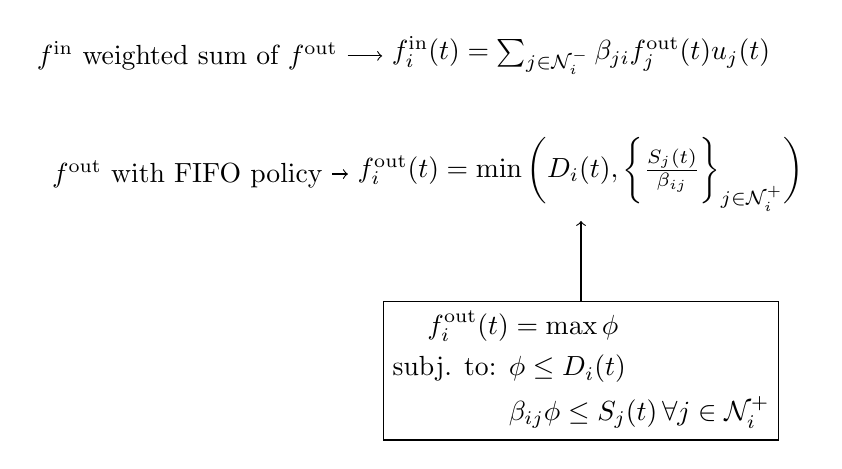
\begin{tikzpicture}
    \uncover<2->{
        \node (sum) at (0,0) {$f^\text{in}$ weighted sum of $f^\text{out}$};
    }
    \uncover<3->{
    \node (fifo) at (0,-1.5) {$f^\text{out}$ with FIFO policy};
    }
    \uncover<3->{
    \node (fout) at (5,-1.5) {$\ptcoly{f^\text{out}_i(t)} = \min\bigg( D_i(t), \bigg\{ \frac{S_j(t)}{\beta_{ij}}\bigg\}_{j\in\neighDown_i} \bigg)$};
    }
    \uncover<2->{
    \node (fin) at (5,0) {$\ptcolx{f^\text{in}_i(t)} = \sum_{j\in\neighUp_i} \beta_{ji}f^\text{out}_j(t)u_j(t)$};
    }
    \uncover<2->{
    \draw[->] (sum)--(fin);
    }
    \uncover<3->{
    \draw[->] (fifo)--(fout);
    }
    \uncover<4->{
    \node[draw] (box) at (5,-4) {%
    $
    \begin{aligned}
    f^\text{out}_i(t) &= \max \phi\\
    \text{subj. to:   } & \phi\leq D_i(t)\\
        & \beta_{ij}\phi\leq S_j(t)\,\forall j\in\neighDown_i
    \end{aligned}
    $
    };
    
    \draw[->] (box)--(fout);
    }
    \end{tikzpicture}
\end{frame} % Flow conservation 

\begin{frame}
    \frametitle{S-CTM - Example}
    \metroset{block=fill}
    \begin{block}{Diverge network}
    \begin{columns}[c]
    \begin{column}{0.4\textwidth}
      \begin{figure}
      \includegraphics[scale=0.6]{fig_51_diverge3}
      \end{figure}
    \end{column}
    \begin{column}{0.4\textwidth}
      $
      \onslide<1->{\dot{\rho}_1 = }
      \dfrac{
      \onslide<2->{f_1^{in} - f_1^{out} }
      \onslide<3->{{\color{blue}u_1(t)} }
      }{L_1}
      $
    \end{column}
    \end{columns}
    \end{block}
    \begin{block}<4->{4--roads intersection}
    \begin{columns}[c]
    \begin{column}{0.3\textwidth}
        \hbox{\hspace{3em}
        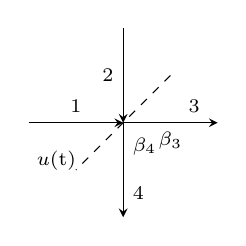
\begin{tikzpicture}[>=stealth,scale=0.6]
        \draw[->] (0,0)--(2,0) node[midway, above, color=black]  {\scriptsize$1$};
        \draw[->] (2,2)--(2,0) node[midway, left, color=black] {\scriptsize$2$};
        \draw[->] (2,0)--(4,0) node[near end, above, color=black] {\scriptsize$3$} node[midway, below, color=black] {\scriptsize $\beta_3$};
        \draw[->] (2,0)--(2,-2) node[near end, right, color=black] {\scriptsize$4$} node[near start, right, color=black] {\scriptsize $\beta_4$};
        \coordinate (a) at (1,-1);
        \coordinate (b) at (3.3,1);
        \draw[dashed] (3,1)--(1,-1) node[above left = -5pt  of a] {\scriptsize$u$(t)};% node[above left = -5pt of b] {$\alpha^{(2)}$};
        \end{tikzpicture}}
    \end{column}
    \begin{column}{0.7\textwidth}
      $
      \dot{\rho}_3 = \frac{1}{L_3} \Big(f_3^{in} - f_3^{out}\Big)  = \frac{ \Big(\big( \onslide<6->{{\color{blue}u_1(t)}} \onslide<5->{{\color{black}f_1^{out}}\beta_{13}} + \onslide<6->{{\color{blue}\big(1-u_1(t)\big)}} \onslide<5->{{\color{black}f_2^{out}\beta_{23}}} \big) - f_3^{out}  \Big)}{L_3}
      $
    \end{column}
    \end{columns}
    \end{block}
\end{frame} % Example intersection 

\begin{frame}
  \frametitle{Model simplification}
  \metroset{block=fill}
  \begin{block}{Why simplification/approximation ? }
  \begin{itemize}
  \item To have a more scalable model (thanks to continuous instead of binary function)
  \item To include duty cycle as a new variable (towards control application)
  \end{itemize}
  \end{block}
  \uncover<2->{
  \begin{block}{Store \& forward method (Aboudolas et al., 2008)}
  Provided that spills are avoided (Demand \&{}Supply paradigm) a flow $f$ becomes
  \begin{columns}[c]
  \column{0.4\textwidth}
  \[
  f = \left\{
  \begin{aligned}
  &0 \mbox{ if } u(t)=0\\
  &\varphi \mbox{ otherwise}
  \end{aligned}
  \right.
  \]  
  \column{0.4\textwidth}
  \includegraphics[scale=0.5]{fig_52_SFM}  
  \end{columns}
  \end{block}
  }
\end{frame} % Model simplification 

\begin{frame}{The average cell transmission model (Avg-CTM)}
    \newcommand*\colavg{} 
    \only<3->{\renewcommand*\colavg{\textcolor{blue}}}
    \metroset{block=fill}
    \begin{block}{Model reduction}
    Can the binary behavior of the S-CTM be simplified?
    \end{block}
    \uncover<2->{
    \begin{minipage}[c]{0.45\textwidth}
    \includegraphics[scale=1]{fig_53_duty}
    \end{minipage}
    \begin{minipage}[c]{0.45\textwidth}
    Compute the average value
    \[
    \colavg{\bar{u}_i(t)} = \frac{1}{T/T_s}\sum_{k=1}^{T/T_s}u_i(t+kT_s)
    \]
    \end{minipage}
    }
    \uncover<3->{
    \[
    \begin{aligned}
    \bar{\rho}_i(t+T_s) &= \bar{\rho}_i(t) + \frac{T_s}{L_i} \bigg( f^\text{in}_i(t) - \colavg{\bar{u}_i(t)} f^\text{out}_i(t) \bigg)\\
    \onslide<4->{
    &\text{subj. to constraints from the S-CTM}\\
    & \forall\, i\in\roads\setminus\roadsin,\, \forall\,t\in\mathbb{N}_+\quad \sum_{j\in\neighUp_i}\colavg{\bar{u}_j(t)}\leq 1.}
    \end{aligned}
    \]
    }
    \uncover<4->{
    \emph{Note:} $\roads\setminus\roadsin$ denote the set of \emph{internal roads} in the network.
    }
\end{frame} % Computing the average

\begin{frame}{Avg-CTM: Example}
    \begin{center}
    
    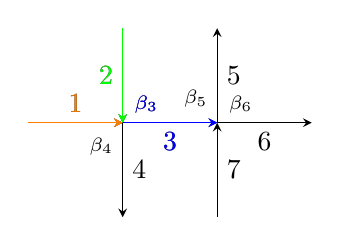
\begin{tikzpicture}[>=stealth,scale=0.6]  
    \draw[->] (0,0)--(2,0) node[midway, above, color=black]  {$1$};
    \uncover<3->{
    \draw[->,orange] (0,0)--(2,0) node[midway, above, color=orange]  {$1$};
    }
    \draw[->] (2,2)--(2,0) node[midway, left, color=black] {$2$};
    \uncover<3->{
    \draw[->,green] (2,2)--(2,0) node[midway, left, color=green] {$2$};
    }
    \draw[->] (2,0)--(4,0) node[midway, below, color=black] {$3$} node[near start, above, color=black] {\scriptsize $\beta_3$};
    \uncover<2->{
    \draw[->,blue] (2,0)--(4,0) node[midway, below, color=blue] {$3$} node[near start, above, color=blue] {\scriptsize $\beta_3$};}
    \draw[->] (2,0)--(2,-2) node[midway, right, color=black] {$4$} node[near start, left, color=black] {\scriptsize $\beta_4$};
    \draw[->] (4,0)--(6,0) node[midway, below, color=black] {$6$} node[near start, above, color=black] {\scriptsize $\beta_6$};
    \draw[->] (4,0)--(4,2) node[midway, right, color=black] {$5$} node[near start, left, color=black] {\scriptsize $\beta_5$};
    \draw[->] (4,-2)--(4,0) node[midway, right, color=black] {$7$} ;
    \end{tikzpicture}
    \end{center}
    \[
    \begin{aligned}
    \onslide<1->{\dfrac{L_3}{T_s}(\overline{\rho_3^+}-\overline{\rho}_3)} &= \onslide<2->{{\color{blue}f_3^{in}} - \Malpha_3 f_3^{out} =} \onslide<3->{{\color{orange}{\Malpha_1}\beta_{13}} f_1^{out} + {\color{green}(1-\Malpha_1)\beta_{23}}f_2^{out} - \Malpha_3 f_3^{out} =} \\
    &
    \begin{aligned}
     \onslide<4->{= \Malpha_1 \beta_{13} \min\bigg\{ D_1, \frac{S_3}{\beta_{13}}, \frac{S_4}{\beta_{14}}\bigg\}} \onslide<5->{&+ (1-\Malpha_1)\beta_3\min\bigg\{ D_2, \frac{S_3}{\beta_{23}}, \frac{S_4}{\beta_{24}}\bigg\}} \\
     \onslide<6->{&- \Malpha_2 \min\bigg\{ D_3, \frac{S_5}{\beta_5}, \frac{S_6}{\beta_6} \bigg\}}
     \end{aligned}
    \end{aligned}
    \]
    \begin{block}{Consistency of the model}
    \begin{itemize}
    \item Total outflow never bigger than inflow
    \item Inflow/outflow respect the Demand \& Supply paradigm
    \end{itemize}
    \end{block}
    \end{frame} % Example average inflow

\begin{frame}{Avg-CTM --- Macroscopic validation}
    \begin{center}
    \resizebox{!}{0.25\textwidth}{
    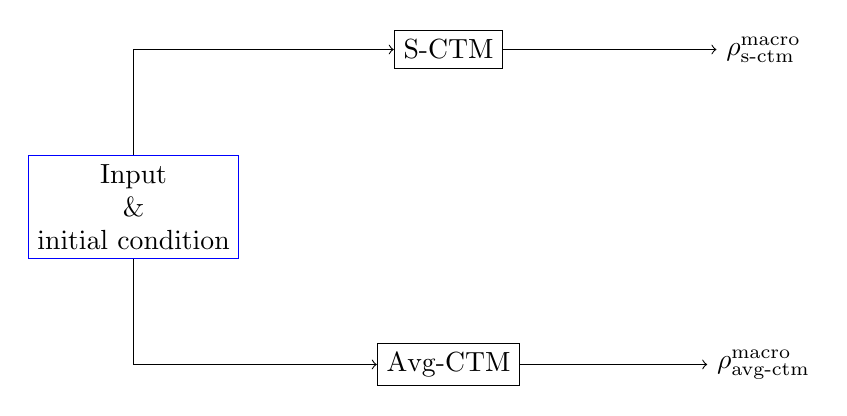
\begin{tikzpicture}
    \node[draw=blue, align=center] (input) at (0,0) {Input \\ \& \\ initial condition};
    \node[draw=black] (sctm) at (4,2) {S-CTM};
    \node[draw=black] (avgctm) at (4,-2) {Avg-CTM};
    \node (s) at (8,2) {$\rho^\text{macro}_\text{s-ctm}$};
    \node (avg) at (8,-2) {$\rho^\text{macro}_\text{avg-ctm}$};
    \draw[->] (input)|-(sctm);
    \draw[->] (input)|-(avgctm);
    \draw[->] (sctm)--(s);
    \draw[->] (avgctm)--(avg);
    \end{tikzpicture}
    }
    \end{center}
    \begin{center}
        \includegraphics[scale=0.45]{fig_54_manhattan4by4}
    \end{center}
\end{frame}
 % Validation via macrosimulation

\begin{frame}{Results --- Macroscopic validation}
    \begin{center}
    \resizebox{!}{0.25\textwidth}{
    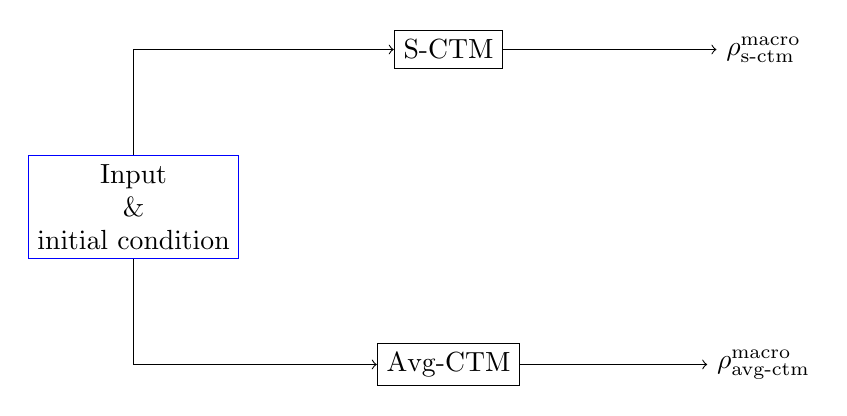
\begin{tikzpicture}
    \node[draw=blue, align=center] (input) at (0,0) {Input \\ \& \\ initial condition};
    \node[draw=black] (sctm) at (4,2) {S-CTM};
    \node[draw=black] (avgctm) at (4,-2) {Avg-CTM};
    \node (s) at (8,2) {$\rho^\text{macro}_\text{s-ctm}$};
    \node (avg) at (8,-2) {$\rho^\text{macro}_\text{avg-ctm}$};
    \draw[->] (input)|-(sctm);
    \draw[->] (input)|-(avgctm);
    \draw[->] (sctm)--(s);
    \draw[->] (avgctm)--(avg);
    \end{tikzpicture}
    }
    \end{center}
    \begin{center}
        \includegraphics[scale=0.45]{fig_55_validationSCTM}%
        \quad%\hspace{1em}%
        \includegraphics[scale=0.45]{fig_56_validationAvgCTM}%
    \end{center}
\end{frame}
 % Results macrosimulation

\begin{frame}
    \frametitle{S-CTM --- Microscopic validation}
    \metroset{block=fill}
    \begin{block}{Validation objective}
    How close is the signalized CTM to a realistic behavior (e.g., microscopic models)?
    \end{block}
    \begin{center}
    \begin{tikzpicture}
    \node[draw=blue, align=center] (input) at (0,0) {Input \\ \& \\ initial condition};
    \node (aimsun) at (4,2) {\includegraphics[scale=0.3]{fig_57_aimsun}};
    \node[draw=black] (sctm) at (4,-2) {S-CTM};
    \node (micro) at (8,2) {$\rho^\text{micro}$};
    \node (macro) at (8,-2) {$\rho^\text{macro}$};
    \draw[->] (input)|-(aimsun);
    \draw[->] (input)|-(sctm);
    \draw[->] (aimsun)--(micro);
    \draw[->] (sctm)--(macro);
    \end{tikzpicture}
    \end{center}
\end{frame} % Validation via microsimulation

\begin{frame}{S-CTM --- Microscopic validation}
    \begin{center}
    \includegraphics[scale=0.17]{fig_58_singleIntersectionAimsun}
    \end{center}
    \begin{center}
    \centering
    \includegraphics[scale=0.4]{fig_59_density329}
    ~
    \includegraphics[scale=0.4]{fig_60_density330}
    ~
    \includegraphics[scale=0.4]{fig_61_density331}
    \end{center}
\end{frame} % Results microsimulation 

\begin{frame}{Comments}
    \begin{itemize}
    \item<1-> The intrinsic complexity of the most descriptive traffic models (microscopic) makes them unsuitable for control synthesis
    \item<2-> We rely on macroscopic representations, starting off with the CTM and extending it to account for signalized intersections (S-CTM)
    \item<3-> The binary dynamics of traffic lights can be approximated with an average trajectory (Avg-CTM) that proves in practice to be a good approximation of the former
    \item<4-> The Avg-CTM is a smoother model, suitable for control design with duty cycle as control variables
    \end{itemize}
    \metroset{block=fill}
    \uncover<5->{
    \begin{block}{Remaining question}
        How to design a control for such a model?
    \end{block}
    }
\end{frame} % Comments and remarks

\begin{frame}{Control history}
    \begin{columns}
    \column{0.5\textwidth}
    \begin{itemize}
      \item \textbf{1772} - Manual of traffic flow control
      \item \textbf{1866} - Heritage from railway systems
      \item \textbf{1960} - Driver Aided Information and Routing (DAIR)
      \item \textbf{1990} - Loop detectors + Message signs
      \item \textbf{1991} - ALINEA
      \item \textbf{2000} - Hierarchical control
      \item \textbf{2010+} - Vehicle focus/ MAAS
    \end{itemize}
    \column{0.5\textwidth}
    \begin{figure}
        \onslide<1->{\includegraphics[scale = 0.4]{fig_62_light-hist.png}}
        \onslide<2>{\includegraphics[width = \textwidth]{fig_63_dair.png}}
    \end{figure}
    \end{columns}
\end{frame} % Control in traffic history

\begin{frame}{Control objective}
    \metroset{block=fill}
    \includegraphics[width=\textwidth]{fig_64_balancing}
    \begin{block}{Objectives of $u$}
    \begin{itemize}
      \item Maximize the throughput of the network.
      \item Homogenize the use of the network (when possible)
    \end{itemize}
    \end{block}
\end{frame} % Control objectives 

\begin{frame}[shrink=8]{Traffic performance metrics}
    \metroset{block=fill}
    \begin{exampleblock}{Total travel distance:}
        Full amount of distance travelled by all vehicles in the network    
        \[
        \text{TTD}(t) = \sum_{k=0}^{\floor{t/T_s}} \sum_{i\in\roads}f_i(kT_s)
        \]
    \end{exampleblock}
    \begin{exampleblock}{Density balancing}
        Notion on how uniformly vehicles spread in the network. Ideally \emph{uniform} vehicle distribution. 
        
        \[
        \text{Bal}(t) = \sum_{k=0}^{\floor{t/T_s}} \sum_{i\in\roads}\sum_{j\in\neighDown_i}(\rho_i(kT_s)-\rho_j(kT_s))^2
        = \sum_{k=0}^{\floor{t/T_s}} \rho'(kT_s)\laplacian\rho(kT_s)
        \]
        
        where
        \[
        \begin{aligned}
        \laplacian_{ii} = \lvert \mathcal{N}_i \rvert, 
        \laplacian_{ij} = \begin{cases} -1 & \text{if } j\in\mathcal{N}_i\\
                    0 & \text{elsewhere.}
            \end{cases}
        \end{aligned}
        \]
    \end{exampleblock}
\end{frame} % Traffic metrics - I


\begin{frame}{Traffic performance metrics}
    \metroset{block=fill}
    \begin{exampleblock}{Traffic signal regularization}
    This intends to reduce strong changes in the control cycle of the traffic signal. 
    \[
    R(\bar{u}(t,T))= \Vert\bar{u}(t)-\bar{u}(t-T)\Vert_2^2
    \]
    \emph{Note:} $T$ represents the full signal cycle period.
    \end{exampleblock}  
    \begin{exampleblock}{Other traffic indicators:}
        \begin{itemize}
        \item Service of demand
        \item Total travel time
        \item Queues length
        \item Stop time
        \end{itemize}
    \end{exampleblock}
\end{frame} % Traffic metrics - II

\begin{frame}{Tools to improve traffic indicators}
    \begin{columns}
    \begin{column}{0.5\textwidth}
    \only<1-2>{
    \begin{exampleblock}{Optimization}
    In order to optimize the \emph{cost} $f(x)$, the value of $x$ should be found, while respecting the constraints
        \begin{equation*}
        x^*=
        \begin{aligned}
        &\underset{x}{\min}& &f(x)\\
        &\text{s.t}& &x\geq0.5
        \end{aligned}
        \end{equation*}
    \end{exampleblock}
    }
    \only<3->{
    \begin{exampleblock}{Design \& Constraints}  
    \begin{itemize}[<+->]
        \item Duty cycle $\bar{u}$ as control variable
        \item Maximize network throughput + minimize the balance
        \item Model-based predictions computed by using the Avg-CTM
    \end{itemize}
    \end{exampleblock}
    }
    \end{column}
    \begin{column}{0.5\textwidth}
    \begin{figure}
    \includegraphics[width=\textwidth]{fig_65_square}
    \end{figure}
    \onslide<2->{
    \begin{exampleblock}{Optimal criteria}
        \[
            \underset{\bar{u}}{\min}\ Bal\left(\bar{u}(t)\right) - TTD\left(\bar{u}(t)\right) + R\left(\bar{u}(t,T)\right)
        \]        
    \end{exampleblock}
    }    
    \end{column}
    \end{columns}


\end{frame} % Control problem idea


\begin{frame}[shrink=9]{Control problem formulation}
    The traffic signal control problem then consists in finding a solution to the following optimization problem:
    \[
    \begin{aligned}
    \min_{\bar{u}} & \quad \sum_{k=1}^{K} \bigg( k_\text{bal}\bar{\rho}'(t+kT_s)\laplacian\bar{\rho}(t+kT_s) -
            k_\text{ttd}\sum_{i\in\roads} f_i(t+kT_s) \bigg)
            + \Vert\bar{u}-\bar{u}(t-T)\Vert_2^2 \\
    & \text{subj. to: } \forall\, i,\, \forall\,t\quad  0\leq\bar{u}_i(t)\leq1\\
                   &\phantom{ \text{subj. to: } \forall\, i,\, \forall\,t\quad} \sum_{j\in\neighUp_i}\bar{u}_j(t)\leq 1.
    \end{aligned}
    \]
    \metroset{block=fill}
    \begin{block}{Control problem characteristics}
        \begin{itemize}
        \item Minimize density balancing
        \item Maximize total travel distance
        \item A convex formulation is achievable when $K=1$
        \end{itemize}
    \end{block}
\end{frame} % Control problem formulation


\begin{frame}<handout:1|beamer:0>
\frametitle{Convexity of the formulation --- ideas}
    \newcommand*\colF{} 
    \only<2>{\renewcommand*\colF{\textcolor{red}}}
    \newcommand*\colQ{} 
    \only<3>{\renewcommand*\colQ{\textcolor{orange}}}
    \newcommand*\colp{} 
    \only<4>{\renewcommand*\colp{\textcolor{blue}}}        
    \begin{itemize}
    \item One step ahead density:
    \begin{equation}
    \bar{\rho}_i(t+T_s) = \bar{\rho}_i(t) + \frac{T_s}{L_i}\bigg(\colF{\sum_{j\in\neighUp_i} \beta_{ji} f^\text{out}_j(t)}\bar{u}_j - \bar{u}_i \colF{f^\text{out}_i(t)}\bigg)
    \end{equation}
    
    \begin{equation}
    \bar{\rho}(t+T_s) = \colF{H(t)} \bar{u} + c(t)
    \end{equation}
    
    \item Bal + regularization:
    \begin{equation}
    \bar{u}^T \colQ{Q} \bar{u} + \colp{p^T} \bar{u}
    \end{equation}
    where
    %
    \begin{equation}
    \colQ{Q = k_\text{bal}H'(t)\laplacian H(t) + I,}
    \end{equation}
    \begin{equation}
    \colp{p = \big( 2 k_\text{bal}c^T(t)\laplacian H(t) - \bar{u}'(t-T) \big)^T.}
    \end{equation}
    \end{itemize}
\end{frame} % Convexity characteristics

\begin{frame}<handout:1|beamer:0>
\frametitle{Convexity of the formulation --- ideas}
    \begin{itemize}
    
    \item Problem formulation (equivalent):
    \[
    \begin{aligned}
    & \min_{\bar{u}}\quad \bar{u}' Q \bar{u} + p' \bar{u} - k_{\text{ttd}}\mathbf{1}'f(\bar{u}) \\
    & \text{subj. to, }\forall i:\, l_i\leq\bar{u}_i\leq 1 \\
    & \phantom{\text{subj. to, }\forall i:\,} \sum_{j\in\neighUp_i}\bar{u}_j \leq 1
    \end{aligned}
    \]
    
    \item The total travel distance can be expressed as a function of $\bar{u}(t)$:
    \begin{multline*}
    f_i(\bar{u}) = \min\Bigg( v_i \bigg( \bar{\rho}_i(t) + \frac{T_s}{L_i}\Big(\sum_{j\in\neighUp_i} \bar{u}_j\beta_{ji} f^\text{out}_j(t) - \bar{u}_i f^\text{out}_i(t) \Big) \bigg), \\
    w_i \bigg( \rho^\text{max}_i - \bar{\rho}_i(t) - \frac{T_s}{L_i}\Big(\sum_{j\in\neighUp_i} \bar{u}_j\beta_{ji} f^\text{out}_j(t) + \bar{u}_i f^\text{out}_i(t) \Big) \bigg) \Bigg).
    \end{multline*}
    \end{itemize}
\end{frame} % Convexity characteristics ii

\begin{frame}<handout:1|beamer:0>
\frametitle{Convexity of the formulation --- ideas}
    \begin{itemize}
    \item Problem formulation (relaxed):
    \[
    \begin{aligned}
    & \min_{\bar{u}, y\geq0}\quad  \bar{u}' Q \bar{u} + p' \bar{u} - k_{\text{ttd}}\mathbf{1}'y \\
    & \text{subj. to, }\forall i:\,  l_i\leq\bar{u}_i\leq1\,\\
    & \phantom{\text{subj. to, }\forall i:\,} \sum_{j\in\neighUp_i}\bar{u}_j \leq 1\\
    & \phantom{\text{subj. to, }\forall i:\,} y_i \leq v_i \bigg( \bar{\rho}_i(t) + \frac{T_s}{L_i}\Big(\sum_{j\in\neighUp_i} \bar{u}_j f^\text{out}_j(t) - \bar{u}_i f^\text{out}_i(t) \Big)\bigg)\\
    & \phantom{\text{subj. to, }\forall i:\,} y_i \leq w_i \bigg( \rho^\text{max}_i - \bar{\rho}_i(t) - \frac{T_s}{L_i}\Big(\sum_{j\in\neighUp_i} \bar{u}_j f^\text{out}_j(t) + \bar{u}_i f^\text{out}_i(t) \Big)\bigg).
    \end{aligned}
    \]
    \end{itemize}
\end{frame} % Convexity characteristics iii

\begin{frame}{Comments}
    \begin{exampleblock}{Observations}
    \begin{itemize}
    \item \textbf{Pros:}
    \begin{itemize}
    \item The relaxed formulation is provably \emph{equivalent} to the original problem
    \item Convex problems are generally considered "easy" to solve
    \end{itemize}
    \item \textbf{Cons:}
    \begin{itemize}
    \item Although efficient, the solution does not scale well with the size of the network
    \end{itemize}
    \end{itemize}
    \end{exampleblock}
    \begin{block}{Remaining question}
        How to design scale the control to large traffic networks?
    \end{block}        
    \uncover<2->{
    \begin{exampleblock}{Scalability requirements}
        \begin{itemize}
            \item Decomposition in subproblems
            \item Communication of efficient information
            \item Iterative and distributed algorithm
            \item Optimality of the distributed algorithm
        \end{itemize}        
    \end{exampleblock}
    }
\end{frame} % Comments and remarks

\begin{frame}{Scalability - Communication graph}
    Minimum information required to determine the solution of a single traffic light $\bar{u}_i$
    \begin{center}
    \includegraphics[scale=0.7]{fig_66_connectivityGraph}
    \end{center}
    Set of roads that can "talk" to $i$:
    \[
    \mathcal{S}_i = \neighUp_i\cup\neighDown_i\cup\mathcal{I}_i,
    \]
    %
    where
    %
    \[
    \mathcal{I}_i = \{q: \neighDown_q \equiv \neighDown_i\}.
    \]
    
    \metroset{block=fill}
    \begin{block}{Why?}
    $\neighUp_i$ and $\neighDown_i$ are needed for density prediction.
    $\mathcal{I}_i$ is needed for constraints over traffic lights.
    \end{block}
\end{frame} % Distribution ideas

\begin{frame}{Scalability - Problem decomposition}
    Problem set-up (e.g., problem $i$):
    \[
    \begin{aligned}
    \min_{\bar{u}}\quad     & \sum_{i\in\roads} g_i \big(\bar{u}^{(i)}_{[p\in\mathcal{S}_i]} \big)\\
    \text{s.t. }          & \bar{u}^{(i)}_{[p\in\mathcal{S}_i]}\in\mathcal{X}_i, \, \forall\, i\in\roads, \\
                          & \bar{u}^{(i)}_i = \bar{u}^{(p)}_i,\quad \forall\, i\in\roads, \, \forall\, p\in\mathcal{S}_i\setminus i \\
                          & \bar{u}^{(i)}_p = \bar{u}^{(p)}_p, \quad \forall\, i\in\roads,\, \forall p\in\mathcal{S}_i\setminus i.
    \end{aligned}
    \]
    %
    where $\bar{u}_p^{(i)}$ is the copy of the global variable $\bar{u}_p$ kept in memory locally by subproblem $i$.
    
    \metroset{block=fill}
    \begin{block}{Why?}
    Each subproblem needs to be self--contained: variables will be requested from others according to the communication graph
    \end{block}
\end{frame} % Problem decomposition

\begin{frame}<handout:1|beamer:0>
    \frametitle{Distributed algorithm}
    Partial (separable) Lagrangian:
    \[
    %\begin{gathered}
    L =\sum_{i\in\roads} L_i =  \sum_{i\in\roads} g_i \big(\bar{u}_{[p\in\mathcal{S}_i]}  \big) +
    %
    \bar{u}_i^{(i)} \sum_{p\in\mathcal{S}_i\setminus i} \big( \lambda_i^{(i,p)} - \lambda_i^{(p,i)} \big) +
    \sum_{p\in\mathcal{S}_i\setminus i} \bar{u}_p^{(i)} \big( \lambda_p^{(i,p)} - \lambda_p^{(p,i)} \big).
    %
    %\end{gathered}
    \]
    \begin{itemize}
    \item[]\textbf{Initialization.} Set $k=0$. Create local variables for each subproblem %$\bar{u}_p$, $\lambda^{(i,p)}_p$, for every $p\in\mathcal{S}_i$
    %
    \item[]\textbf{Primal update.} Update primal variables $\bar{u}_p(k+1)$ by minimizing the $i$-th term of the partial Lagrangian
    %
    \item[]\textbf{Transmission.} Send primal local variables to requiring neighbors $p\in\mathcal{S}_i$, and collect the most recent values of $\bar{u}_i^{(p)}$, $\bar{u}_p^{(p)}$ from them
    \item[]\textbf{Dual update.} Update the Lagrangian multipliers with a gradient update of step $\alpha$
    %
    \item[]\textbf{Stop condition.} If the solution has numerically stabilized then stop, otherwise increment $k$ and go to 1
    \end{itemize}
\end{frame} % Distributed algorithm

\begin{frame}{Numerical simulations}
    \begin{exampleblock}{Two-fold evaluation}
    \begin{itemize}
    \item Time to convergence of the distributed algorithm
    \begin{itemize}
    \item Number of iteration before the iterative procedure stabilizes, measured in different numerical scenarios
    \end{itemize}
    \end{itemize}
    
    \begin{itemize}
    \item Traffic performance
    \begin{itemize}
        \item Measure of traffic metrics, both macroscopic and microscopic
    \end{itemize}
    \item Simulation setup
    \begin{itemize}
        \item Several network dimensions (from 4 to 180 roads)
        \item Initial state randomly selected (in 300 simulations)
        \end{itemize}
    \end{itemize}
    \end{exampleblock}
\end{frame} % Numerical simulation setup

\begin{frame}{Traffic performance}
    \begin{itemize}
    \item Comparisons with a best practice (BP) schedule, chosen to optimize the statistical traffic behavior
    \end{itemize}
    
    \begin{center}
        \begin{minipage}[c]{0.45\textwidth}
        \includegraphics[scale=0.5]{fig_67_density}%
        \end{minipage}
        ~
        \begin{minipage}[c]{0.45\textwidth}
        %\centering
        \includegraphics[scale=0.5]{fig_68_densityFeedback}%
        \end{minipage}%
    \end{center}
\end{frame} % Density indicators (open-closed loop) comparisson

\begin{frame}{Traffic performance}
    \begin{center}
        \begin{minipage}[c]{0.45\textwidth}
        %\centering%
        \includegraphics[scale=0.5]{fig_71_TTD}%
        \end{minipage}
        ~
        \begin{minipage}[c]{0.3\textwidth}
        %\centering
        \includegraphics[scale=0.5]{fig_69_balancingCost}%
        \end{minipage}%
    \end{center}
    \begin{center}
        \includegraphics[scale=0.5]{fig_70_SoD}
    \end{center}
\end{frame} % Performance indicators

\begin{frame}{Miscroscopic simulation}
    \centering{
    \includegraphics[scale=0.15]{fig_72_aimsunCity}
    }
    \smallskip
    \centering{\small
    \begin{tabular}{ccccc}
    \toprule
    Index & \multicolumn{2}{c}{Scenario 1} & \multicolumn{2}{c}{Scenario 2}\\
    \cmidrule(lr){2-3}
    \cmidrule(lr){4-5}
     & BP & OSA-TC & BP & OSA-TC\\
    \midrule
    Travelled distance [km] & 23396 & 26471 & 19772 & 17003\\
    Travel time [h] & 1775 & 1462 & 1955 & 1583 \\
    Mean queue [veh] & 496 & 441 & 627 & 564\\
    Stop time [sec/km] & 123 & 97 & 172 & 139\\
    \bottomrule
    \end{tabular}
    }
\end{frame} % Microscopic scenario

\begin{frame}{Scenario description - Case study Grenoble}
\begin{center}
\includegraphics[scale=0.55]{fig_73_LineC}
\end{center}
\end{frame} % Scenario picture

\begin{frame}{Scenario description}
    \begin{exampleblock}{General characteristics}
    \begin{itemize}
    \item Intersection are equipped with several on--off detectors
    \item Every intersection is controlled by a single--intersection controller
    \item A fusion of data from GPS and magnetic detectors is used in order to say to the controller how far the trams are
    \item Several constant parameters (min/max green time, amber time) are decided as function of the speed limit, the number and size of lanes, the size of the intersections
    \end{itemize}
    \end{exampleblock}
\end{frame}
 % Scenario description

\begin{frame}{Grenoble traffic lights plan (plan de feux)}
    \begin{center}
        \centering
        \includegraphics[scale=0.55]{fig_74_flowChartPdF}
    \end{center}
    \begin{center}
        \includegraphics[scale=0.55]{fig_75_PdF}
    \end{center}
\end{frame}
 % Real traffic lights behavior

\begin{frame}{Numerical comparisons}
    \begin{exampleblock}{General characteristics - Light traffic plan}
    Set up:
    \begin{itemize}
    \item Traffic lights plan virtually replicated into Aimsun
    \item Input flow and supply estimated by real data extracted by loop detectors\dots
    \item \dots as well as split ratios at intersections\dots
    \item \dots from 7am to 10am
    \item Adaptation of the OSA-TC to fit this scenario's technological requirements
    \item A posteriori analysis of on--line measured data (within Aimsun)
    \end{itemize}
    \end{exampleblock}
\end{frame} % Real traffic lights scenario


\begin{frame}{Numerical results}
    \begin{center}
    \scalebox{0.7}{%
    \begin{tabular}{ccc}
    \toprule
    Index & Plan de feux & Optimal control \\
    \midrule
    Input flow [veh/h] & 6097 & 6151\\
    Mean queue [veh] & 152 & 113\\
    Stop time [sec/km] & 110 & 83\\
    TTD [km] & 16307 & 16411\\
    TTT [h] & 794 & 680\\
    Veh. waiting [veh] & 333 & 240\\
    \bottomrule
    \end{tabular}
    }
    \end{center}
    \begin{center}
    \includegraphics[scale=0.6]{fig_76_queueTotalPdF}
    \end{center}
    \end{frame}
    
    \begin{frame}{Numerical results}
    \begin{center}
    \includegraphics[scale=0.8]{fig_77_travelTimeDouble}
    \end{center}
    \end{frame}
    
    \begin{frame}{Numerical results}
    \begin{center}
    \includegraphics[scale=0.8]{fig_78_travelTimeSingle}
    \end{center}
\end{frame}
 % Numerical results

\begin{frame}{Final comments}
    \begin{itemize}
    \item We have designed an optimization--based algorithm to control green split of traffic lights
    \item The control algorithm is applicable to large cities thanks to its scalability property
    \item Numerical simulations show the improvements w.r.t. standard fixed--time policies
    \item The algorithm can be adapted to real scenarios and in simulations it performs better than "real world" traffic lights scheduling algorithms
    \end{itemize}
\end{frame}
 % Final comments

\section{Connected vehicles}


\begin{frame}
\frametitle{Classical Vehicles}
    \metroset{block=fill}
    \begin{center}
        \resizebox{0.9\linewidth}{!}{%
            \includestandalone[width=0.9\linewidth]{fig_79_classical_vehicle}
        }
        \begin{exampleblock}{Features}
            \begin{itemize}
                \item Perception only from the driver's perspective
                \item Local information only available 
                \item Poor accuracy on observed data
            \end{itemize}
        \end{exampleblock}
    \end{center}
\end{frame} % Regular vehicles 

\begin{frame}
\frametitle{Equipped Vehicles}
    \metroset{block=fill}
    \begin{center}
        \resizebox{0.9\linewidth}{!}{%
            \includestandalone{fig_80_equipped_vehicle}
        }
        \begin{exampleblock}{Features}
            \begin{itemize}
                \item Improved perception via radar sensors
                \item Speed regulation via Adaptive Cruise Control (ACC)
                \item Only longitudinal information 
            \end{itemize}
        \end{exampleblock}
    \end{center}
\end{frame} % Eqquiped vehicles 

\begin{frame}
\frametitle{Connected Vehicles - V2I}
    \metroset{block=fill}
    \begin{center}
        \resizebox{0.9\linewidth}{!}{%
            \includestandalone{fig_81_connected_vehicle}
        }
        \begin{exampleblock}{Features}
            \begin{itemize}
                \item Improved perception via communication with other vehicles
                \item Accuracy on information depend on external sensors
                \item Longitudinal + lateral information 
            \end{itemize}
        \end{exampleblock}
    \end{center}
\end{frame} % Connected vehicle

\begin{frame}
\frametitle{Connected Vehicles - V2I}
    \metroset{block=fill}
    \begin{center}
        \resizebox{0.9\linewidth}{!}{%
            \includestandalone{fig_82_connected_vehicle_RSU}
        }
        \begin{exampleblock}{Features}
            \begin{itemize}
                \item Non local information from infrastructure 
                \item Local information (longitudinal + lateral)
                \item Accuracy limited by data provided via V2V/V2I
            \end{itemize}
        \end{exampleblock}
    \end{center}
\end{frame} % Connected vehicle RSU\

\begin{frame}
\frametitle{Smart Vehicles}
    \metroset{block=fill}
    \begin{center}
        \resizebox{0.9\linewidth}{!}{%
            \includestandalone{fig_83_intelligent_vehicle}
        }
        \begin{exampleblock}{Features}
            \begin{itemize}
                \item Local and non local information leveraged by V2X communications
                \item Improved possibility for better automation (ACC/CACC)
            \end{itemize}
        \end{exampleblock}
    \end{center}
\end{frame} % Smart vehicle

\begin{frame}
    \frametitle{Smart Vehicles}
    What could be the potential impact of those connected vehicles?
    \begin{center}
        \begin{figure}
            \includegraphics[width=0.75\textwidth]{fig_85_cav_effects_traffic}
            \caption{Impact of connected vehicles on traffic}
        \end{figure}
    \end{center}
    \begin{alertblock}{Features}
        \begin{itemize}
            \item They contribute as \emph{sensors} for current traffic condition
            \item They can adapt to traffic conditions known in advance
            \item They can cooperate to inform other users about current road situation. 
        \end{itemize}
    \end{alertblock}
\end{frame} % CAV in traffic  

\begin{frame}
    \frametitle{SCOOP Scenario}

    \begin{center}
        \resizebox{0.8\linewidth}{!}{%
            \includegraphics{fig_84_test_scoop}
        }
    \end{center}
    \begin{alertblock}{Sensitivity analysis}
        \begin{itemize}
            \item Emission distance of broadcasted messages
            \item Speed drop message 
            \item Demand 
            \item Market penetration rate  
        \end{itemize}
    \end{alertblock}    
\end{frame}
 % SCOOP Test 

\begin{frame}<handout:0|beamer:1>
\frametitle{Simulation Example SymuVia}
\begin{center}
    \includemedia[width=\linewidth,activate=pageopen,
    passcontext,
    transparent,
    addresource=video/SCOOP_final_fast.mp4,
    flashvars={source=video/SCOOP_final_fast.mp4}
    ]{\includegraphics[width=0.9\linewidth]{fig_90_video_scoop}}{VPlayer.swf}
\end{center}
\end{frame}
 % Video SCOOP

\begin{frame}
\frametitle{Results in terms of Market Penetration Rate}
Spatial distribution of congestion is better achieved at higher \emph{penetration rates}, effects of works are better avoided. Nevertheless, increasing the \emph{penetration rate} may also have an impact on the \emph{network throughput}.
\begin{center}
\begin{columns}
    \begin{column}{0.3\textwidth}
    \begin{figure}
        \centering
        \includegraphics[width =1.15\textwidth]{fig_86_xt_mpr10}
        \caption{MPR = $10\%$}
    \end{figure}
    \end{column}
    \begin{column}{0.3\textwidth}
        \begin{figure}
            \centering
            \includegraphics[width = 1.15\textwidth]{fig_87_xt_mpr20}
            \caption{MPR = $20\%$}
        \end{figure}
    \end{column}
    \begin{column}{0.3\textwidth}
        \begin{figure}
            \centering
            \includegraphics[width = 1.15\textwidth]{fig_88_xt_mpr30}
            \caption{MPR = $30\%$}
        \end{figure}
    \end{column}
\end{columns}
\end{center}
\end{frame} % Results spacing 

\begin{frame}
\frametitle{Potential impact of Connected vehicles}
Earlier messages may potentially increase the impact of CO$_2$ emissions. The \emph{market penetration rate} is an important factor that may also reduce the impact on CO$_2$ emissions.
    \begin{figure}
        \centering
        \includegraphics[width =0.9\textwidth]{fig_89_CO2vsFlow}
        \caption{Relative change in CO$_2$ emissions with SCOOP technolgies}
    \end{figure}
\end{frame} % CO 2 savings 

\begin{frame}
    \frametitle{Conclusions \& Observations}
    \metroset{block=fill}
    \begin{block}{To takeaway}
    \begin{itemize}
        \item Introduction of V2V/V2I may have a potential impact on traffic safety, road operation efficiency and emissions.
        \item Speed drop policies may conduct to optimal absorption of traffic effects
        \item Market penetration rate itself constitute an important factor for potential environmental impacts. 
    \end{itemize}
    \end{block}
    \uncover<2->{
    \begin{block}{Current research directions}
        \begin{itemize}
            \item Analyzing the impact of delayed acceptation on policies and the effect of anarchy. 
            \item Non-uniform market penetration rates.  
        \end{itemize}
    \end{block}
    }
\end{frame} % Conclusions 

\section{Vehicle platooning}

% \begin{frame}<handout:0|beamer:1>
    \frametitle{Truck platooning}
    \begin{center}
        \includemedia[width=\linewidth,activate=pageopen,
        passcontext,
        transparent,
        addresource=video/platooning.mp4,
        flashvars={source=video/platooning.mp4}
        ]{\includegraphics[width=0.9\linewidth]{fig_91_platooning}}{VPlayer.swf}
    \end{center}
\end{frame}
 % Video Platooning

\begin{frame}
    \frametitle{Dynamic traffic assingment - Problem}
    \begin{columns}
      \begin{column}{0.5\textwidth}
        \begin{figure}
          \includegraphics[width=0.8\linewidth]{fig_22_intersection}
        \end{figure}
      \end{column}
      \begin{column}{0.5\textwidth}
        \begin{block}{Questions}
          How to assign the flow at time \(t\)?
        \end{block}
        Some key principles\footcite{Coclite:2005}: 
        \begin{enumerate}
          \item Flow conservation 
          \item Flow maximization
          \item Infrastructure limitations
          \item Set/calibrate drivers' preferences
        \end{enumerate}
      \end{column}
    \end{columns}
    Unless the drivers preferences are well known the solution to the DTA problem is undetermined. 
\end{frame} % Dynamic traffic assignment intro


\begin{frame}
  \frametitle{Dynamic traffic assignment at Merges}
  \begin{columns}
    \begin{column}{0.5\textwidth}
      Let consider the case: 
      \begin{equation*}
        \begin{aligned}
        \onslide<4->{&\underset{f_i}{\max}& &\sum f_i\\}
        \onslide<1->{&\text{s.t} & & f_1 \leq D_1  \\}
        \onslide<2->{& & & f_2 \leq D_2\\}
        \onslide<3->{& & & f_1 + f_2 \leq S_3}
        \end{aligned}
      \end{equation*}
      \uncover<4-:>{
      \begin{block}{Solution}
        In general the dynamic traffic assingment problem has multiple values \(f_1,f_2\) that may satisfy the problem constraints.
      \end{block}
      }
    \end{column}
    \begin{column}{0.5\textwidth}
      \begin{figure}
        \includegraphics[width=0.8\linewidth]{fig_23b_merge.pdf}
      \end{figure}
      \only<1|handout:0>{
        \begin{figure}
          \includegraphics[width=0.8\linewidth]{fig_24a_diagram_merge}
        \end{figure}
      }
      \only<2|handout:0>{
        \begin{figure}
          \includegraphics[width=0.8\linewidth]{fig_24b_diagram_merge}
        \end{figure}
      }
      \only<3|handout:0>{
        \begin{figure}
          \includegraphics[width=0.8\linewidth]{fig_24c_diagram_merge}
        \end{figure}
      }
      \only<4|handout:1>{
        \begin{figure}
          \includegraphics[width=0.8\linewidth]{fig_24d_diagram_merge}
        \end{figure}
      }
    \end{column}
  \end{columns}    
\end{frame} % DTA problem solution

\begin{frame}
    \frametitle{Control of vehicle distance in vehicles (ADAS)}
    \tikzstyle{block} = [draw, fill=blue!20, rectangle, minimum height=3em, minimum width=6em]
    \tikzstyle{system} = [draw, fill=red!20, rectangle, minimum height=3em, minimum width=6em]
    \tikzstyle{interface} = [draw, fill=green!20, rectangle, minimum height=3em, minimum width=6em]
    \tikzstyle{sum} = [draw, fill=blue!20, circle, node distance=1cm]
    \tikzstyle{input} = [coordinate]
    \tikzstyle{output} = [coordinate]
    \tikzstyle{pinstyle} = [pin edge={to-,thin,black}]
    \begin{center}
    \begin{tikzpicture}[auto, node distance=2cm,>=latex']
      \node [block] (controller) {Controller};
      \node [interface, right of=controller,node distance=2.5cm] (actuator) {Throttle};
      \node [system, right of=actuator, pin={[pinstyle]above:Disturbances}, node distance=4cm] (system) {Vehicle};
      \draw [->] (controller) -- node[name=u] {$u$} (actuator);
      \draw [->] (actuator) -- node[name=u] {$u_a$} (system);
      \node [output, right of=system, node distance = 2.5cm] (output) {};
      \node [interface, below of=u] (measurements) {Sensors};
      \draw [->] (system) -- node [name=y] {$y = s$}(output);
      \draw [->] (y) |- (measurements);
      \draw [->] (measurements) -| node[pos=0.99] {}
    node [near end] {$y_m$} (controller);
    \end{tikzpicture}
    \end{center}
    \begin{columns}
    \begin{column}{0.5\textwidth}
    \begin{itemize}
      \item $u$ - Required acceleration
      \item $u_a$ - Gas pedal 
      \item $y$ - Inter vehicle distance
    \end{itemize}
    \end{column}
    \begin{column}{0.5\textwidth}
      \begin{exampleblock}{Objective}
      \begin{itemize}
        \item Regulate the headway space between two vehicles.
        \item Adapt to dynamic condition of the leader.
    \end{itemize}
      \end{exampleblock}
    \end{column}
    \end{columns}
\end{frame} % Truck platoon control objective

\begin{frame}{Context on vehicle platooning}
\metroset{block=fill}
    Truck platooning has some ideas in mind: 
      \begin{itemize}[<+->]
        \item \textbf{Objective}: Improve fuel consumption in trucks 
        \item \textbf{Traffic issues}: 
        \begin{itemize}
          \item String stability \(\rightarrow\) flow stability.
          \item Interactions at network discontinuities \(\rightarrow\) Capacity drop. 
        \end{itemize}  
      \end{itemize}
      \onslide<4->{There however still some concerns regarding interaction between them and the reality}
      \begin{block}<5->{Objective}
        The main objective today is to propose a strategies for \structure{promoting  Connected \& Automated Vehicles maneuvers} at network discontinuities. 
      \end{block}
    \end{frame} % Objective of today


\begin{frame}
    \frametitle{Human Driven - Car following model}
    \begin{columns}
    \begin{column}{0.5\textwidth}
      \begin{figure}
        \includegraphics[width=0.8\linewidth]{fig_2_time_space}
      \end{figure}
      \uncover<2-|handout:1>{
      \begin{equation*}
        \scriptsize
        \begin{aligned}
          x_i(t) = \min(x^F_i(t),x^C_i(t))\\
          \begin{cases}
            x^F_{i}(t)= x_i(t-\tau) + u \tau \\
            x^C_{i}(t)= x_{i-1}(t-\tau) - \delta
          \end{cases}
        \end{aligned}
      \end{equation*}
      }
    \end{column}
    \begin{column}{0.7\textwidth}
      \begin{center}
      \uncover<3-|handout:1>{
      \begin{itemize}
      \item Truck properties
        \begin{itemize}
          \item[\(L\)] Vehicle's length 
          \item[\(u\)] Free flow speed 
          \item[\(\kappa_x\)] Maximum density
        \end{itemize}
      % \onslide<2->{Truck properties}
      \item Platoon properties 
        \begin{itemize}
          \item[\(N\)] Number of trucks 
          \item[\(g_t\)] Time gap policy
        \end{itemize}
      % \onslide<3->{Time headway inside the platoon (front to front)}
      \item Time headway: \(h^p = g^t + L/u\)
      \end{itemize}
      }
      \only<2-3|handout:0>{
      \begin{figure}
          \includegraphics[width=0.6\linewidth]{fig_1a_fund_diag.pdf}\hspace*{2cm} 
      \end{figure}
      }
      \only<4|handout:0>{
      \begin{figure}
        \includegraphics[width=0.6\linewidth]{fig_1b_fund_diag.pdf}\hspace*{2cm} 
      \end{figure}
      }
      \only<5|handout:0>{
      \begin{figure}
        \includegraphics[width=0.6\linewidth]{fig_1c_fund_diag.pdf}\hspace*{2cm} 
      \end{figure}
      }
      \only<6|handout:1>{
      \begin{figure}
        \includegraphics[width=0.6\linewidth]{fig_1d_fund_diag.pdf}\hspace*{2cm} 
      \end{figure}
      }
    \end{center}
    \end{column}
      \end{columns}
  \end{frame} % Regular driver's model


\begin{frame}
    \frametitle{Low speed insertion Problems  \footcite{Duret2010:TRB}}
    \begin{columns}
      \begin{column}{0.5\linewidth}
        \begin{figure}
          \includegraphics[width=0.8\linewidth]{fig_3_low_speed.pdf}
          \caption{\scriptsize Low speed wave propagation}
        \end{figure}
      \end{column}
      \begin{column}{0.5\linewidth}
        \begin{itemize}[<+->]
          \item Low safety 
          \item Shockwave initiation
          \item Transition period until equilibirum 
          \item This may create capacity drop  
        \end{itemize}
        \onslide<5->{
        \begin{block}{Proposal}
          It is necessary to anticipate for truck platoons to \structure{anticipate} these maneuvers.
        \end{block}
        }
      \end{column}
    \end{columns}
\end{frame}
 % Research problem

\begin{frame}
\frametitle{Truck platoon models near a merge}
\metroset{block=fill}
    \smartdiagramset{description title width=1.2cm, 
            description title text width=2cm}
    \onslide<1->{        
    \begin{columns}
      \begin{column}{0.6\linewidth}
        \smartdiagram[descriptive diagram]{
          {\textit{\textbf{Assumption}},{\structure{V2V/V2I} full connectivity}},
          {\textit{\textbf{Objective}}, {\structure{Safety} at the merge condition, + \alert{smoothed traffic} in main lane/ carrigeway}},
        }
      \end{column}
      \begin{column}{0.2\linewidth}
        \begin{figure}
          \includegraphics[width=\linewidth]
          {fig_25_truck-platoon-cutin}
        \end{figure}
      \end{column}
    \end{columns}
    }
    \onslide<2->{
    \begin{block}{Anticipated maneuver}
      \begin{description}
        \item[Detection] Measurement / detection of vehicles far upstream 
        \item[Yielding] Coordinated deccelearation between all trucks. 
        \item[Insertion] Smooth insertion   
      \end{description}
    \end{block}
    }
\end{frame}
 % Platoon near merges


\begin{frame}
    \frametitle{Maneuver execution}
    The maneuver is executed via a \structure{bi-level} control strategy\footcite{Duret2018a:JMT}:
    \begin{description}
      \item[Tactical layer]  Takes decision at the traffic level.  
      \item[Operational layer] Operates vehicles and control its acceleration. 
    \end{description}
    \vspace{-1cm}
    \begin{columns}
      \begin{column}{0.5\textwidth}
          \only<1|handout:0>{
          \begin{figure}
              \includegraphics[width=\linewidth]{fig_5a_merge-phases.pdf}\hspace*{2cm} 
          \end{figure}
          }
          \only<2|handout:0>{
          \begin{figure}
            \includegraphics[width=\linewidth]{fig_5b_merge-phases.pdf}\hspace*{2cm} 
          \end{figure}
          }
          \only<3|handout:1>{
          \begin{figure}
            \includegraphics[width=\linewidth]{fig_5c_merge-phases.pdf}\hspace*{2cm} 
          \end{figure}
          }
      \end{column}
      \begin{column}{0.5\textwidth}
        \begin{figure}
          \includegraphics[width=0.9\linewidth]{fig_6_bilevel-strategy.pdf}\hspace*{2cm} 
        \end{figure}
      \end{column}
    \end{columns}
\end{frame} % Idea for coordinated merge

\begin{frame}
    \frametitle{Important aspects in maneuver executions}
    \metroset{block=fill}
      This maneuver can be executed in multiple ways, 
      \begin{itemize}
        \item \only<1|handout:0>{\footnotesize\structure{\cite{Ntousakis2016:TR-C,Rios-Torres2017a:TITS}}} Designed focused on trajectory planning problem. 
        \item \structure{Mixed traffic}. It is a key important factor for the controllability of the system. 
      \end{itemize}
      \begin{columns}
        \column{0.3\textwidth}
        \uncover<1->{
          \textbf{Inputs}
          \begin{itemize}
            \item[\(T_m\)] merging time
            \item[\(X_m\)] merging position
            \item[\(u\)] merging speed 
          \end{itemize}
          }
        \column{0.4\textwidth}
        \uncover<2->{
          \textbf{Parameters}
          \begin{itemize}
            \item[\(\varepsilon\)] maximum speed drop
            \item[\(a^{-/+}\)] maximum acceleration.
          \end{itemize}
          }
        \column{0.35\textwidth}
        \uncover<3->{
          \textbf{Decision variables}
          \begin{itemize}
            \item[\(i\)] Truck index
            \item[\(T_a\)] anticipation time
          \end{itemize}
          }       
      \end{columns}
      \uncover<4->{
      \begin{block}{Mixed traffic assumption}
        Regarding the mixed traffic \(w = \underbrace{\delta_p/ \tau_p}_{\text{\tiny CAV}} = \underbrace{\delta/ \tau}_{\text{\tiny HDV}}\)
      \end{block}
      }
\end{frame}
 % Aspects in the maneuver execution


\begin{frame}
    \frametitle[Before]{Vehicle merging case I: CAV environment}
    \textbf{Before}
    \centering
      \only<1|handout:0>{
      \begin{figure}
          \includegraphics[width=0.9\linewidth]{fig_7a_merge_cav_bef.pdf}\hspace*{1cm} 
      \end{figure}
      }
      \only<2|handout:0>{
      \begin{figure}
        \includegraphics[width=0.9\linewidth]{fig_7b_merge_cav_bef.pdf}\hspace*{1cm}
      \end{figure}
      }
      \only<3|handout:1>{
      \begin{figure}
        \includegraphics[width=0.9\linewidth]{fig_7c_merge_cav_bef.pdf}\hspace*{1cm}
      \end{figure}
      }
  \end{frame} % Case Full CAV - I

\begin{frame}
    \frametitle[After]{Vehicle merging case I: CAV environment}
    \textbf{After}
    \centering
      \only<1|handout:0>{
      \begin{figure}
          \includegraphics[width=0.9\linewidth]{fig_8a_merge_cav_aft.pdf}\hspace*{1cm} 
      \end{figure}
      }
      \only<2|handout:0>{
      \begin{figure}
        \includegraphics[width=0.9\linewidth]{fig_8b_merge_cav_aft.pdf}\hspace*{1cm}
      \end{figure}
      }
      \only<3|handout:1>{
      \begin{figure}
        \includegraphics[width=0.9\linewidth]{fig_8c_merge_cav_aft.pdf}\hspace*{1cm}
      \end{figure}
      }
  \end{frame} % Case Full CAV - II

\begin{frame}
    \frametitle[Before]{Vehicle merging case II: Mixed environment}
    \textbf{Before}
    \centering
      \only<1|handout:0>{
      \begin{figure}
          \includegraphics[width=0.9\linewidth]{fig_9a_merge_mixed_bef.pdf}\hspace*{1cm} 
      \end{figure}
      }
      \only<2|handout:0>{
      \begin{figure}
        \includegraphics[width=0.9\linewidth]{fig_9b_merge_mixed_bef.pdf}\hspace*{1cm}
      \end{figure}
      }
      \only<3|handout:1>{
      \begin{figure}
        \includegraphics[width=0.9\linewidth]{fig_9c_merge_mixed_bef.pdf}\hspace*{1cm}
      \end{figure}
      }
  \end{frame}
 % Case Mixed Traffic I

\begin{frame}
    \frametitle[After]{Vehicle merging case I: CAV environment}
    \textbf{After}
    \centering
      \only<1|handout:0>{
      \begin{figure}
          \includegraphics[width=0.9\linewidth]{fig_9a_merge_mixed_aft.pdf}\hspace*{1cm} 
      \end{figure}
      }
      \only<2|handout:0>{
      \begin{figure}
        \includegraphics[width=0.9\linewidth]{fig_9b_merge_mixed_aft.pdf}\hspace*{1cm}
      \end{figure}
      }
      \only<3|handout:1>{
      \begin{figure}
        \includegraphics[width=0.9\linewidth]{fig_9c_merge_mixed_aft.pdf}\hspace*{1cm}
      \end{figure}
      }
  \end{frame} % Case Mixed Traffic - II

\begin{frame}
\frametitle{Vehicle merging - summary}
\metroset{block=fill}
    \uncover<1->{
    \begin{block}{Finding intersections with congestion wave}
    Let \(g^\ell_k = \begin{pmatrix}x^\ell_k & t^\ell_k\end{pmatrix}^T\) if \(p(g^\ell_k)\): projection to the shockwave \(w\)
      \begin{equation*}
        \begin{pmatrix}
          p_x(g^\ell_k)\\
          p_t(g^\ell_k)
        \end{pmatrix} = 
        \frac{1}{u+w}
        \begin{bmatrix}
           1 & u\\
           -1 & w 
        \end{bmatrix}
        \left(
        \begin{pmatrix}
          X_m\\
          x_\ell^{k}
        \end{pmatrix} + 
        \begin{bmatrix}
          w & 0\\
          0 & -u
        \end{bmatrix}
        \begin{pmatrix}
          T^0_m\\
          t^{\ell}_k
        \end{pmatrix}
        \right)
      \end{equation*}
    \end{block}}
    \uncover<2->{
    \begin{block}{CAV}
      The \emph{a-priori} order is obtained by organizing the full set of projections \(\mathcal{P} = \{p(g^{\ell^+}_{1}), \dots, p(g^{\ell^+}_{n+m})\}\)
    \end{block}
    }
    \uncover<3->{
    \begin{block}{Mixed case}
      The problem in this case can be as a \structure{resource allocation} problem. Vehicles can be allocated between two internal boundary conditions \(j_k, j_{k+1}\) as: 
      \begin{equation*}
        \eta \leq \floor*{\left(\Delta\tau^f_{{j_k},{j_{k+1}}}-2\tau\right) / \tau_p}+1
      \end{equation*}
    \end{block}
    }
  \end{frame} % Merging summary (computation)

\begin{frame}
    \frametitle{Transient Period}
    \centering
      \only<1|handout:0>{
      \begin{figure}
          \includegraphics[width=0.9\linewidth]{fig_10a_dyn_split.pdf}\hspace*{1cm} 
      \end{figure}
      }
      \only<2|handout:0>{
      \begin{figure}
        \includegraphics[width=0.9\linewidth]{fig_10b_dyn_split.pdf}\hspace*{1cm}
      \end{figure}
      }
      \only<3|handout:0>{
      \begin{figure}
          \includegraphics[width=0.9\linewidth]{fig_10c_dyn_split.pdf}\hspace*{1cm} 
      \end{figure}
      }
      \only<4|handout:0>{
      \begin{figure}
        \includegraphics[width=0.9\linewidth]{fig_10d_dyn_split.pdf}\hspace*{1cm}
      \end{figure}
      }
      \only<5|handout:0>{
      \begin{figure}
          \includegraphics[width=0.9\linewidth]{fig_10e_dyn_split.pdf}\hspace*{1cm} 
      \end{figure}
      }
      \only<6|handout:1>{
      \begin{figure}
        \includegraphics[width=0.9\linewidth]{fig_10f_dyn_split.pdf}\hspace*{1cm}
      \end{figure}
      }         
  \end{frame} % Transient period 


\begin{frame}
    \frametitle{Transient period: Anticipation time}
    \begin{equation*}
      T_a = \frac{\epsilon}{2}\left(\frac{1}{a^+}- \frac{1}{a^-}\right) + \frac{u+w}{\epsilon}(T^f_{\sigma_x}-T^{0}_{\sigma_x})
    \end{equation*}
    \textbf{Parameter detail}
    \begin{table}
      \begin{tabular}{l | c }
      Parameter Name & Description \\
      \hline \hline
      \(T^f_{\sigma_x}, T^0_{\sigma_x}\)  & Time shifts leader/follower  \onslide<2-> \\ 
      \(\epsilon\) & Speed drop \onslide<3->\\
      \(u,w\) & Free flow/ shockwave speeds \onslide<4->\\
      \(a^+,a^-\) & Bounding accelerations
      \end{tabular}
      \caption{Parameter dependence}
    \end{table}
  \end{frame} % Anticipation time


\begin{frame}
    \frametitle{Transient period: Decision chart}
    \begin{equation*}
      T_a = \frac{\epsilon}{2}\left(\frac{1}{a^+}- \frac{1}{a^-}\right) + \frac{u+w}{\epsilon}(T^f_{\sigma_x}-T^{0}_{\sigma_x})
    \end{equation*}
  
    \begin{columns}
      \column{0.5\textwidth}
      \uncover<-1>{  
      \textbf{Anticipation Time}
        \begin{figure}
          \includegraphics[width=0.9\linewidth]{fig_11a_anticipation_time.pdf}\hspace*{1cm}
        \end{figure}
      }
      \column{0.5\textwidth}
      \uncover<-1>{
      \textbf{Speed drop}
        \begin{figure}
          \includegraphics[width=0.9\linewidth]{fig_11b_anticipation_time.pdf}\hspace*{1cm}
        \end{figure}
      }
    \end{columns}
  \end{frame} % Anticipation time (Decision chart)


\begin{frame}
    \frametitle{Operational layer}
    \begin{figure}
      \centering
      \includegraphics[width=0.7\linewidth]{fig_15_CAV_HDV_follow.png}
      \caption{Mixed traffic scenario}
    \end{figure}
    \begin{itemize}[<+->]
      \item Available measurements for a vehicle: 
      \begin{itemize}
       \item[\(s_k\)] Headway space 
       \item[\(v_k\)] Vehicle's speed
       \item[\(v_{k-1}\)] Leader's speed
      \end{itemize}
      \item Consideration of \structure{3rd order} linear dynamics. 
        \begin{equation*}
          x_i(s) = \left(\frac{1}{s}\right)\left(\frac{1}{s+b}\right)\left(\frac{1/T_e}{s+1/T_e}\right)
        \end{equation*}
    \end{itemize}
\end{frame} % Operational layer (model)


\begin{frame}
    \frametitle{Operational layer}
    \uncover<1->{
    \begin{block}{Model Predictive Control}
      \begin{itemize}
        \item Integration of optimality \structure{safety}, \structure{comfort} + model constraints. 
        \item Predictive feauture for CAVs until the merging position.
      \end{itemize}
    \end{block}
    }
    \uncover<2->{
    \begin{block}{Vehicle's dynamics}
      \begin{equation*}
      \dot{\mathbf{x}}(t) = \frac{d}{dt}\begin{pmatrix}\mathbf{e}_s & \mathbf{e}_v\end{pmatrix} \rightarrow \text{LTI system} + \mathbf{a} \in\ [a^-,a^+]
      \end{equation*}
    \end{block}
    }
    \uncover<3->{
    \begin{block}{Cost function}
      \begin{equation*}
        \mathcal{L}(\mathbf{e}_s,\mathbf{e}_v,\mathbf{a}) = \sum^n_{k=1}\underbrace{c_1\left(s_k-s^r_k\right)^2}_{\text{\tiny Safety}} \onslide<2->{+ \underbrace{c_2\left(v_{k-1}-v_k\right)^2}_{\text{\tiny \color{blue}Homogeneity}}+} \onslide<3>{\underbrace{c_3a^2_k}_{\text{\tiny \color{red} Comfort}}}
      \end{equation*}
      \textbf{Note}: For this case the control can eventually be distributed.
    \end{block}
    }
  \end{frame} % Operational layer (control)


\begin{frame}
    \frametitle{Full control strategy deployment}
    Decisions require \(T_a\), amount of time and the desired time gap (headway space) that should be opened. 
    Constant time gap policy \(s = s_0 + h v\)
    \vspace{0.5cm}
    \begin{center}
    \only<1|handout:0>{
    \begin{figure}
      \includegraphics[width=0.8\linewidth]{fig_12a_control_strategy_deploy.pdf}
      % \caption{Tactical-Operational block diagram}
    \end{figure}
    }
    \only<2|handout:1>{
    \begin{figure}
      \includegraphics[width=0.8\linewidth]{fig_12b_control_strategy_deploy.pdf}
      % \caption{Tactical-Operational block diagram}
    \end{figure}
    }         
    \end{center}
    \vspace{-1cm}
    \textbf{Note:} Gap policy at equilibrium will depend on the leader after merge.
  \end{frame} % Full control strategy

\begin{frame}
    \frametitle{Experimental setup}
    \begin{example}
      \textbf{Scenario}
      \begin{itemize}
        \item Single merge 
        \item 8 CAV vehicles on the main lane: \structure{Platoon in equilibrium conditions}
        \item 2 HDV vehicles on the onramp: \structure{HDV in free flow condition}
      \end{itemize}
    \end{example}
\end{frame}
 % Scenario description

\begin{frame}
    \frametitle{Operational layer performance}
    \begin{columns}
      \begin{column}{0.5\textwidth}
        \begin{figure}
          \centering
          \includegraphics[width=0.9\linewidth]{fig_17_accelerations_vehicles.pdf}
          \caption{Control signal}
        \end{figure}
      \end{column}
      \begin{column}{0.5\textwidth}
        \begin{figure}
          \centering
          \includegraphics[width=0.9\linewidth]{fig_18_reference_low_level.pdf}
          \caption{Time gap reference}
        \end{figure}
      \end{column}
    \end{columns}
\end{frame} % Operational control performance

\begin{frame}
    \frametitle{Operational layer performance - model mismatch}
    \begin{columns}
      \begin{column}{0.5\textwidth}
        \begin{figure}
          \centering
          \includegraphics[width=0.9\linewidth]{fig_16a_model-mismatch.pdf}
          \caption{Vehicle's reference}
        \end{figure}
      \end{column}
      \begin{column}{0.5\textwidth}
        \begin{figure}
          \centering
          \includegraphics[width=0.9\linewidth]{fig_16b_model-mismatch.pdf}
          \caption{Space-time plane}
        \end{figure}
      \end{column}
    \end{columns}
\end{frame} % Robustness of the strategy

\begin{frame}
    \frametitle{Operational layer performance - Delay effects }
      \begin{figure}
        \centering
        \includegraphics[width=0.7\linewidth]{fig_19_delay_effect.pdf}
        \caption{Vehicle's reference}
      \end{figure}
    Lag compensation in the actuator, via the cost function~\footcite{Wang2018:TransportmetricaB}.
\end{frame} % String stability

\begin{frame}
    \frametitle{Case I - CAV scenario}
    \begin{figure}
      \centering
      \includegraphics[width=0.7\linewidth]{fig_14_trajectories_vehiclesCAV.png}
      \caption{Mixed traffic scenario}
    \end{figure}
\end{frame} % Full CAV scenario

\begin{frame}
  \frametitle{Case II - Mixed traffic scenario}
  \begin{figure}
    \centering
    \includegraphics[width=0.7\linewidth]{fig_13_trajectories_vehicles_HDV.png}
    \caption{Mixed traffic scenario}
  \end{figure}
\end{frame} % Mixed scenarios


\begin{frame}
  \frametitle{Results}
  Yielding $T_y$ and anticipation time $T_a$ in seconds
  \begin{table}[bth]
    \begin{threeparttable}
      \begin{tabularx}{\textwidth}{@{}l*{7}{c}@{}}
        \toprule
        &
        \multicolumn{3}{c}{\bfseries Full CAV} &
        \multicolumn{3}{c}{\bfseries Mixed scenario}\\ % note use of "c@{}"
        \cmidrule(lr){2-4} \cmidrule(lr){5-7}  % left- and right-trimming
        Vehicle index \(i_k\) & 
        \multicolumn{1}{L}{\( T_y\)} & 
        \multicolumn{1}{L}{\( T_a\)} & 
        \multicolumn{1}{L}{\(\scriptscriptstyle \scrpt{T}{f}{\sigma_x} - \scrpt{T}{0}{\sigma_x}\)} & 
        \multicolumn{1}{L}{\( T_y\)} & 
        \multicolumn{1}{L}{\( T_a\)} & 
        \multicolumn{1}{L}{\(\scriptscriptstyle \scrpt{T}{f}{\sigma_x} - \scrpt{T}{0}{\sigma_x}\)}\\  % note use of "L@{}"
        \midrule
        $i_3$ & 37.1 & 9.16 & 1.0 & 37.3 & 8.83 & 0.91\\
        $i_5$ & 39.6 & 9.18 & 0.0 & 36.4 & 13.77 & 1.18 \\
        $j_1$ (merging) & 34.4 & 8.60 & 0.86 & N/A & N/A & N/A\\
        $i_7$ & 37.9 & 13.33 & 1.0 & N/A & N/A & N/A\\
        $j_2$ (merging) & 38.0 & 11.99 & 0.81 & N/A & N/A & N/A\\
        \bottomrule
      \end{tabularx}
      \caption{Vehicle index to be relaxed - Anticipation times}
    \end{threeparttable}
  \end{table}
\end{frame}
 % Table comparisons

\begin{frame}
    \frametitle{Conclusions \& Observations}
    \metroset{block=fill}
        \begin{block}{To takeaway}
          \begin{itemize}
            \item Bi-level controllers: Flexible, suitable for integration. 
            \item A method to \structure{safely} split vehicle/truck platoons.
                  \begin{itemize}
                    \item Safe + comfortable gap 
                    \item Smooth trajectories
                  \end{itemize} 
            \item A solution for low speed insertions empowered by anticipation. 
            \item Formulation within an optimal framework. 
          \end{itemize}
        \end{block}
        \begin{block}{Open problems}
        \begin{itemize}
          \item Large flow considerations, in particular the combination.
          \item Merging point \(\rightarrow\) Merging zones.
          \item Uncertainty within the \structure{tactical} layer.
        \end{itemize}
        \end{block}
\end{frame} % Conclusions 

{\setbeamercolor{palette primary}{fg=yellow, bg=black!20}
\begin{frame}[standout]
  Questions?
\end{frame}
} % Questions

\input{82} % Bibliography



\end{document}